% Chapter Template

\chapter{Estudio de resistencia} % Main chapter title
\label{ChapterDESTRUCCION}  % Change X to a consecutive number; for referencing this chapter elsewhere, use \ref{ChapterX}

La resistencia de una red mutualista ante circunstancias adversas, como enfermedades o catástrofes naturales, tiene una gran trascendencia práctica. Las políticas de conservación necesitan basarse en datos que permitan predecir el efecto sobre la comunidad de la pérdida de determinadas especies o de la introducción de otras previamente desaparecidas. Para ello, hay que poder medir la importancia de cada especie para la supervivencia de la red total, o de las especies de una de las clases.

En este capítulo se expone como las \textit{k-magnitudes} pueden contribuir a este propósito, al proporcionar criterios de ordenación con un enfoque novedoso.

%----------------------------------------------------------------------------------------
%	SECTION 1
%----------------------------------------------------------------------------------------

\section{Medición de la resistencia}

La resistencia de una red ecológica es un concepto difícil de precisar \cite{arnoldi2016resilience}. En términos muy generales puede entenderse como la capacidad de supervivencia del sistema ante eventos adversos. Esta definición no resulta satisfactoria si no puede concretarse en una magnitud objetiva. El problema se presenta al escoger la propiedad medible y el método de perturbación. No es lo mismo estudiar la dinámica de las poblaciones ante perturbaciones temporales, que los cambios en la estructura de la red si desaparecen especies o interacciones. Tampoco se obtiene el mismo índice si se miden el tamaño de la componente gigante resultante, el número de especies o el número total de individuos. Por eso, al hablar de resistencia de las comunidades mutualistas, es imprescindible definir con rigor qué se va a medir y cómo se va a alterar la red original.

Pueden distinguirse dos grandes líneas en el estudio de la resistencia. La más extendida es la estática, se modifica la red eliminando nodos, o más raramente enlaces, y se mide cuantas especies sobreviven \cite{memmott2004tolerance, ebenman2005using, kaiser2010robustness}. Esta forma de trabajar se heredó de la investigación sobre \textit{food webs}, que recordemos que son unipartitas \cite{dunne2002biodiversity, dunne2009cascading}. Para estas comunidades se ha usado la \textit{conectancia} como parámetro de estudio, pero como ya se expuso en la introducción es poco descriptivo en el mutualismo.
El método más habitual se basa en provocar extinciones primarias en una de las clases de especies, normalmente en los animales, y medir su efecto sobre la clase contraria.

La otra forma de abordar el problema consiste en perturbar modelos dinámicos o estadísticos y medir el efecto sobre las poblaciones \cite{thebault2010stability, saavedra2013estimating, suweis2013emergence}. Estos procedimientos son más complejos de simular. En un trabajo reciente Gao \textit{et al.} llevan a cabo un estudio analítico de la resistencia de las redes complejas definiendo una \textit{resilience function} que reduce la dimensionalidad del problema y utilizan el modelo II de dinámica mutualista como ejemplo \cite{gao2016universal}. 

La aproximación estática es más simple y es la que seguiremos en este capítulo, pero es necesario señalar sus principales limitaciones. Una es suponer que una especie desaparece solo cuando pierde todos sus enlaces. Esto es evidente en el caso de las especialistas puras que dependen de una sola benefactora para sobrevivir, pero no lo es tanto cuando reciben beneficio de varias pero no con la misma intensidad. El otro gran inconveniente es manejar la red como una entidad inalterable. La extinción de una especie puede hacer que otras a las que desplazaba en el consumo de recursos se puedan aprovechar de los que deja libres. Este tipo de recableado natural ocurre en la naturaleza y altera las condiciones de partida \cite{ramos2012topological, Goldstein2016, timoteo2016high}.

En este tipo de simulaciones es crucial el orden de extinción. No es lo mismo retirar cinco especies al azar que las cinco más conectadas, pero el resultado tampoco es el mismo según el orden con el que se extingan estas cinco. La identificación de las secuencias que resultan más peligrosas para la red es cuestión de investigación abierta \cite{allesina2009googling, dominguez2015ranking}.

\section{Métodos}

En este trabajo hemos usado dos procedimientos de medida de la resistencia según la aproximación estática. En el primero, se ordenan las especies según uno de los criterios que se explicarán a continuación y se van retirando una a una de mayor a menor. No se hace distinción entre clases, pueden producirse extinciones primarias tanto de animales como de plantas. El resultado que se mide es el tamaño de la componente gigante resultante y qué fracción representa de la componente gigante original. El procedimiento se detiene cuando este es la mitad o menos y se registra el número de extinciones primarias que han conducido a ese punto. Se puede comparar la eficacia de los distintos criterios de ordenación sobre la colección de redes midiendo el porcentaje que ese número de especies representa sobre dicha componente original.

El propósito de esta medida es comprobar la resistencia de la red de una manera global. La supervivencia de los fragmentos que puedan quedar aislados de la componente gigante no es crítica para la de la red, porque estamos suponiendo que no hay recableado y que por tanto no se vuelven a conectar.

Los índices de ordenación son: $grado$, ${k}_{degree}$, $centralidad$ $del$ $vector$ $propio$ y ${k}_{risk}$. Los dos primeros ya han aparecido en los capítulos precedentes. La centralidad del vector propio mide la importancia del nodo de una red por la de sus vecinos y se calcula como el vector propio de la matriz de adyacencia \cite{newman2008mathematics}. En nuestra implementación se ha usado la función \texttt{evcent} del paquete \texttt{igrah} de \texttt{R}.

El último índice que utilizaremos es una nueva \textit{k magnitud}, que se añade a definidas en \ref{sec:ESTATICA_defkmagnitudes}. 

\begin{theo} 
El índice \textit{$k_{risk}$} de la especie $m$ de la clase $A$ mide el riesgo relativo para la red que supondría su extinción.
\begin{align*}
k^A_{risk}\left(m\right) = \sum\limits_{i} a_{mi} \left(k^A_{shell}\left(m\right) - k^B_{shell}\left(i\right)\right)\quad   m \in A, \forall i\: in B, k^B_{shell}\left(i\right) < k^A_{shell}\left(m\right)
\end{align*}
\label{krisk}
\end{theo}

Mide el peligro que tiene la desaparición del nodo para las especies que se conectan a él. Si la especie conectada pertenece a una \textit{shell} superior, la desaparición del enlace no es muy grave porque dispondrá de otras fuentes alternativas de beneficio mutualista. Si es de la misma \textit{shell} aplicamos el mismo razonamiento. No es válido si ambas especies son de la $1$-$shell$ pero en ese caso se trata de nodos periféricos que no representan un gran peligro para la red en conjunto.

Para las especies de \textit{shells} inferiores conectadas a la potencialmente extinguida el peligro se incrementa cuanto mayor es la diferencia de los índices $k$. Eso indica una mayor especialización y que el enlace es posiblemente parte del camino más corto a la \textit{shell} máxima.

Es un índice relativo porque sirve para ordenar los nodos de una red, pero no es válido para hacer comparaciones con otras redes. Al ser un ordinal tampoco tiene sentido definir un $k_{risk}$ medio. La pequeña red de dispersores $028$ sirve de ejemplo para explicar el cálculo de esta magnitud (figura \ref{fig:RES_M_SD_028_ziggurat}).

\begin{figure}[h!]
\centering
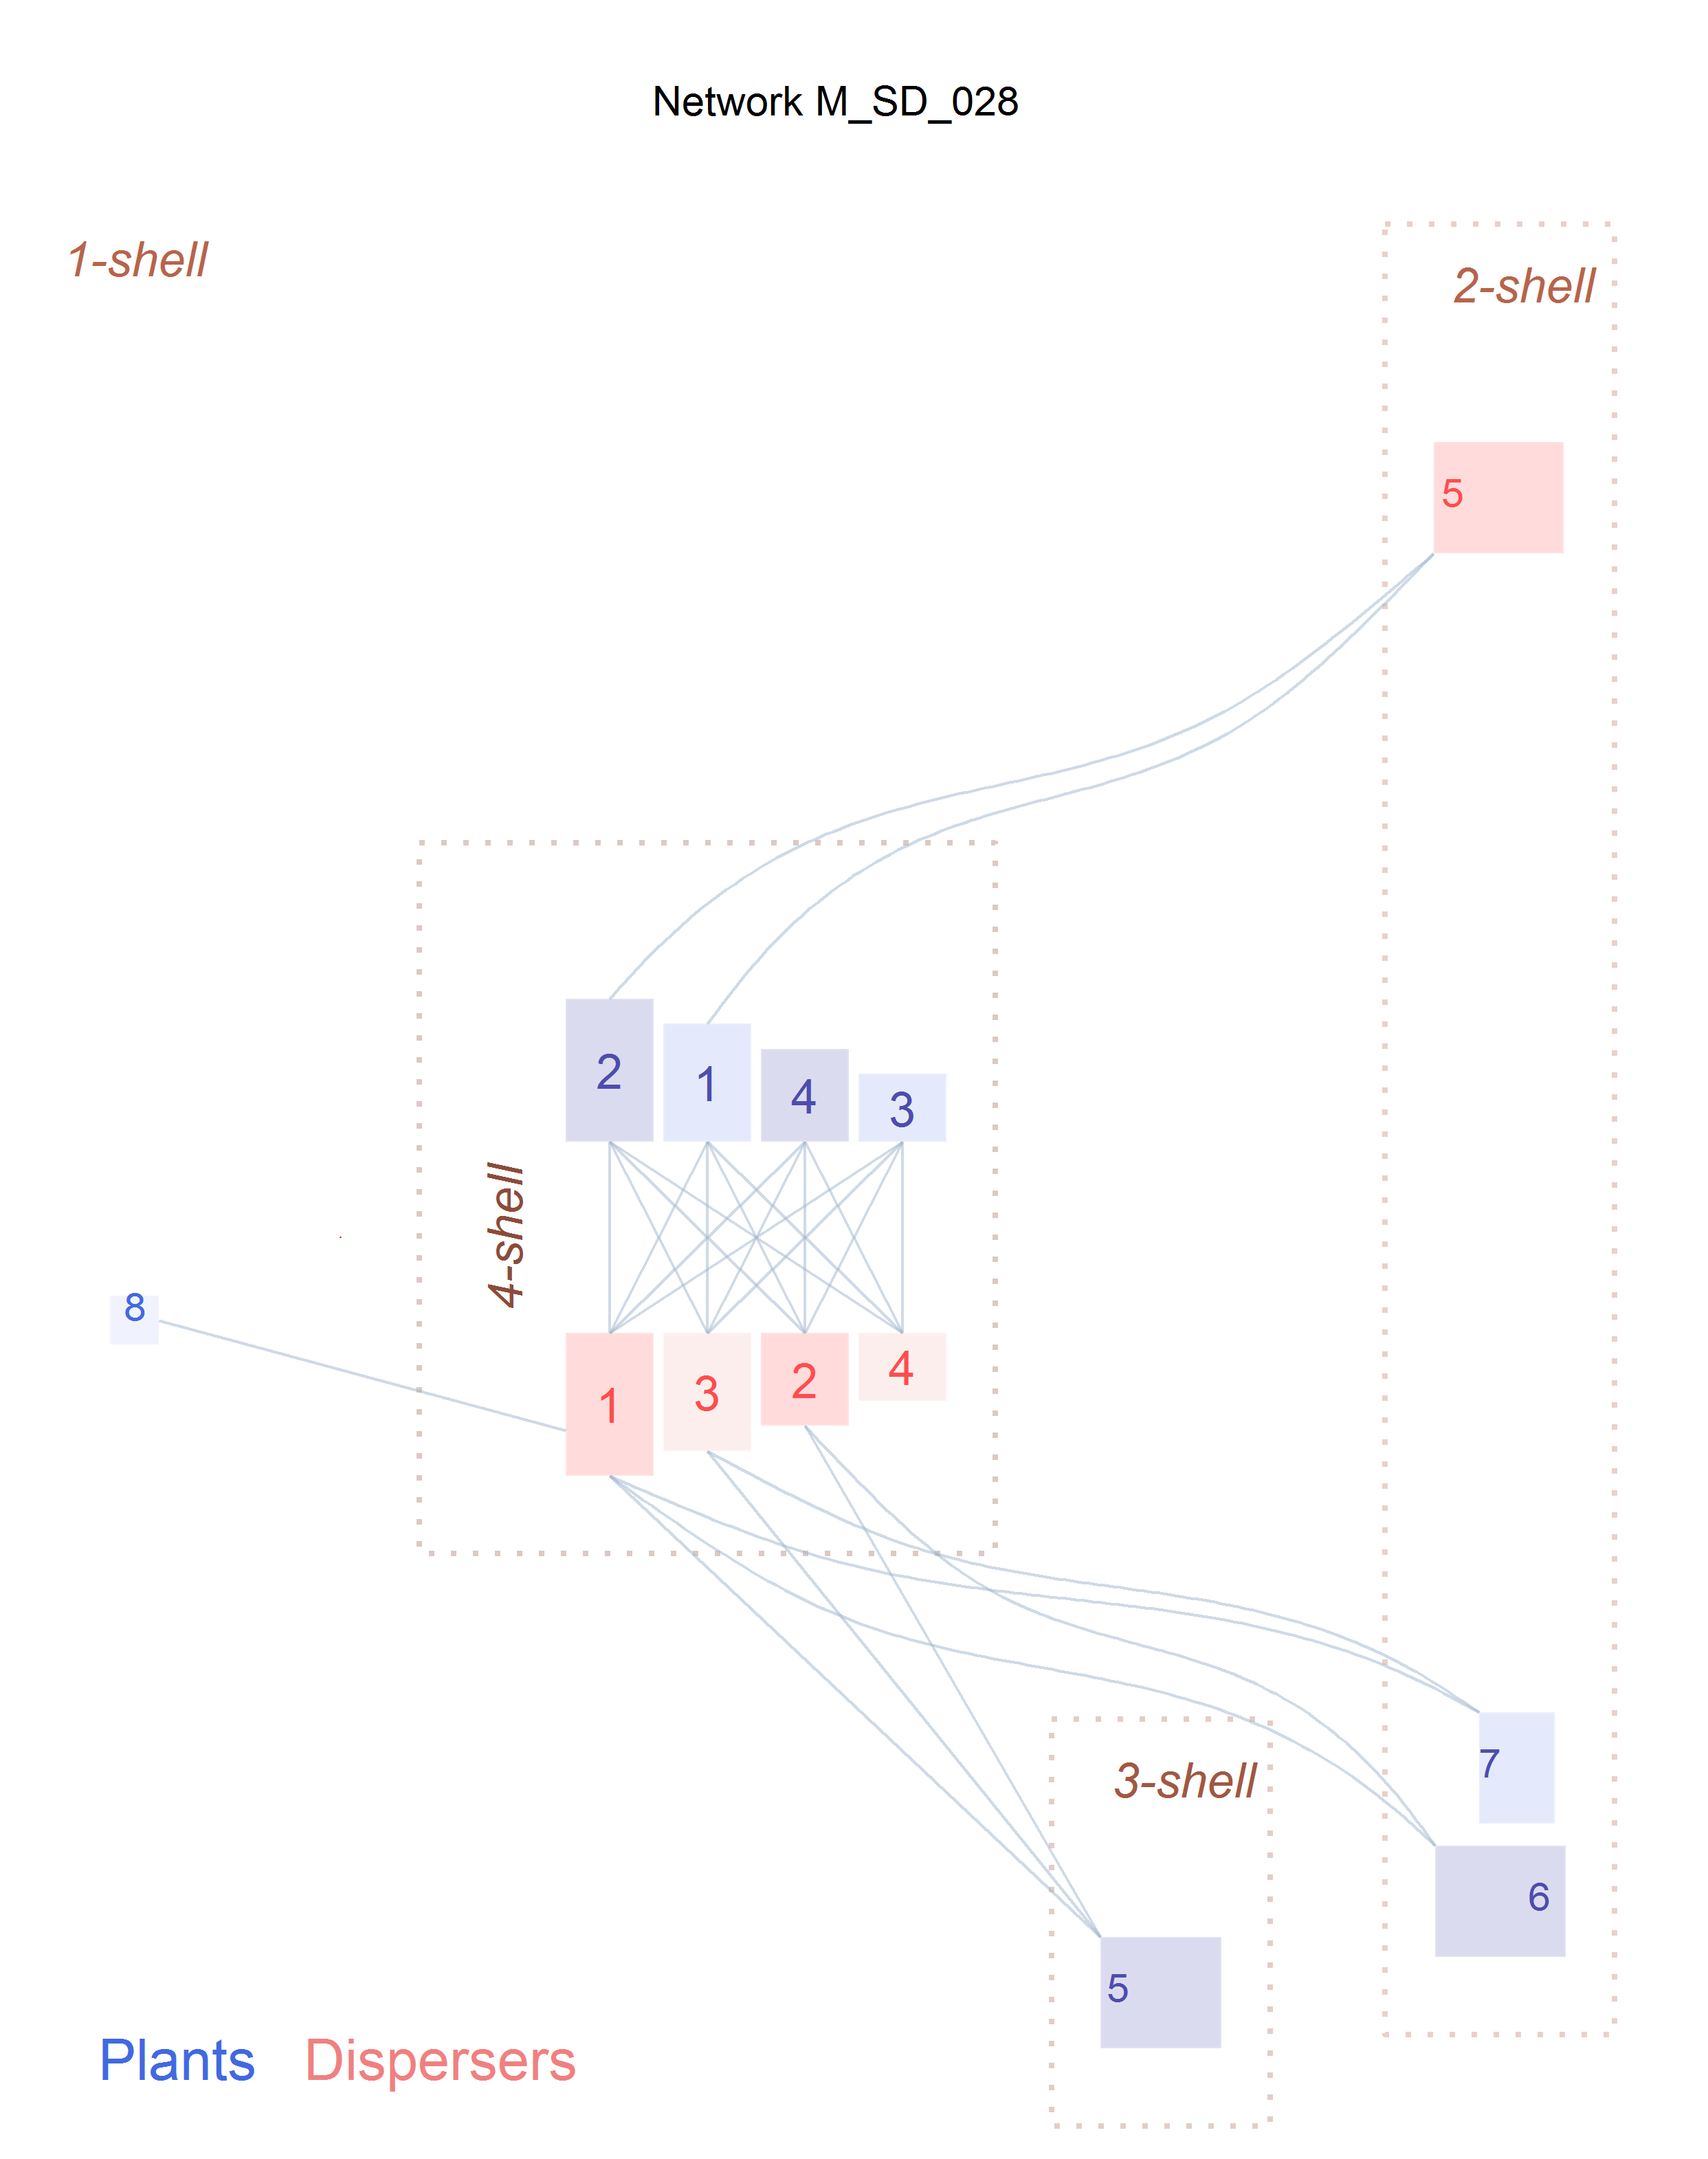
\includegraphics[scale=0.5]{Figures/RES_M_SD_028_ziggurat.png}
\caption{Diagrama zigurat de una de dispersores en la Cañada Travina, Sierra de Cazorla. Compilada por Pedro Jordano, no publicada.}
\label{fig:RES_M_SD_028_ziggurat}
\end{figure}

La planta $2$ que pertenece a la \textit{shell} máxima solo tiene conexión a una especie de índice $k$ inferior, el dispersor $5$ de la $2$-$shell$. Por tanto:

\begin{equation}
k^A_{risk}\left(2\right) = k^A_{shell}\left(2\right) - k^B_{shell}\left(5\right) = 2
\label{krisk_example}
\end{equation}

Algo más elaborado pero no complicado es el cálculo de esta magnitud para el dispersor $1$:

\begin{flalign}
k^B_{risk}\left(1\right) &= k^B_{shell}\left(1\right) - k^A_{shell}\left(8\right) + k^B_{shell}\left(1\right) - k^A_{shell}\left(5\right) + &&\nonumber\\
                         &\,\,\,\,k^B_{shell}\left(1\right) - k^A_{shell}\left(6\right) + k^B_{shell}\left(1\right) - k^A_{shell}\left(7\right) = 3 + 1 + 2 + 2 = 8&&
\label{eq:krisk_example}
\end{flalign}

En la tabla \ref{tab:pars_SD_028} pueden verse los valores de los cuatro índices para toda la red. Como se trata de una comunidad pequeña no hay diferencias importantes
al ordenar por uno u otro criterio, pero en redes mayores sí se producen y tienen consecuencias como se verá en la sección de resultados.



% Table generated by Excel2LaTeX from sheet 'M_SD_028_analysis'
\begin{table}[htbp]
  \centering
  \caption{Parámetros de la red de dispersores $028$.}
  \normalsize
    \begin{tabular}{lrrrrrr}
    \toprule
    $Especie$ & $k shell$ & ${k}_{radius}$ & ${k}_{degree}$ & ${k}_{risk}$ & $degree$ & $eigenc$ \\
\midrule
    pl1  & 4    & 1    & 4,50 & 2    & 5    & 0,32 \\
    pl2  & 4    & 1    & 4,50 & 2    & 5    & 0,32 \\
    pl3  & 4    & 1    & 4,00 & 0    & 4    & 0,29 \\
    pl4  & 4    & 1    & 4,00 & 0    & 4    & 0,29 \\
    pl5  & 3    & 1,5  & 3,00 & 0    & 3    & 0,24 \\
    pl6  & 2    & 2    & 2,00 & 0    & 2    & 0,16 \\
    pl7  & 2    & 2    & 2,00 & 0    & 2    & 0,16 \\
    pl8  & 1    & 2,5  & 1,00 & 0    & 1    & 0,09 \\
    disp1 & 4    & 1    & 6,07 & 8    & 8    & 0,40 \\
    disp2 & 4    & 1    & 5,17 & 3    & 6    & 0,35 \\
    disp3 & 4    & 1    & 5,17 & 3    & 6    & 0,35 \\
    disp4 & 4    & 1    & 4,00 & 0    & 4    & 0,27 \\
    disp5 & 2    & 2    & 2,00 & 0    & 2    & 0,14 \\
    \bottomrule
    \end{tabular}%
      \label{tab:pars_SD_028}%
\end{table}%

El segundo método de destrucción que se aplica en este estudio es el más común. Se provocan extinciones en las especies animales y eso desencadena extinciones secundarias, tanto en las plantas como en otras especies animales que puedan verse arrastradas en cascada. 
En el eje horizontal se representa el porcentaje de especies animales que se extinguen (Figura \ref{fig:DEST_M_PL_001_MRdunne_extinction_plot}). En el vertical, la fracción de la magnitud que se mide. El área normalizada bajo la curva será menor cuanto más rápidamente se reduzca esta últimas como consecuencia de las extinciones primarias. El índice más eficaz para destruir la red es el que da lugar al área menor. El uso de áreas normalizadas permite comparar el comportamiento de dos redes a pesar de sus diferentes estructuras y tamaños.

En el experimento se miden dos magnitudes resultantes:

\begin{enumerate}
\item Fracción de especies de planta que sobreviven, con independencia de que estén o no en la componente gigante.
\item Fracción que queda de la componente gigante original. Se considera que la componente gigante se ha destruido por completo cuando el índice $k$ máximo es $1$.
\end{enumerate}

El orden lo proporcionan los mismos índices que en el experimento anterior, más \textit{MusRank} \cite{dominguez2015ranking}. Este algoritmo no lineal se basa en una adaptación de la idea del algoritmo \textit{PageRank} a redes bipartitas \cite{tacchella2012new}. Se definen dos índices, el de importancia de las especies activas (animales) y el de vulnerabilidad de las pasivas (plantas).

\begin{align}
\tilde{I}^{(n)}_{A} =  \sum\limits_{P=1}^{{P}_{max}} {M}_{AP} {V}^{(n-1)}_{P} \rightarrow  {I}^{(n)}_{A} = \frac{\tilde{I}^{(n)}_{A}}{ {\Bigg \langle \tilde{I}^{(n)}_{A} \Bigg \rangle}_{A} }
\nonumber\\ 
\tilde{V}^{(n)}_{P} =  \frac{1}{\sum\limits_{A=1}^{{A}_{max}} {M}_{AP} \frac{1}{{I}^{(n-1)}_{A}} } \rightarrow  {V}^{(n)}_{P} = \frac{\tilde{V}^{(n)}_{P}}{ {\Bigg \langle \tilde{V}^{(n)}_{P} \Bigg \rangle}_{P} }
\stepcounter{equation}\tag{\theequation}\label{eq:DEST_MusRank}
\end{align}

Donde $\tilde{I}^{(n)}_{A}$ y $\tilde{V}^{(n)}_{P}$ son los valores de dichos índices en la iteración $n$ y ${M}_{AP}$ la matriz de adyacencia que se trata siempre como binaria. El índice de importancia se calcula como el sumatorio de los índices de vulnerabilidad de las especies conectadas en la iteración anterior. El de vulnerabilidad es la inversa del sumatorio de los inversos de los índices de importancia. En cada iteración, las variables $\tilde{I}^{(n)}_{A}$ y $\tilde{V}^{(n)}_{P}$ se normalizan. El algoritmo comienza asignando el valor $1$ a todos los índices. Mediante el procedimiento iterativo terminan convergiendo. Los autores no proporcionan una prueba estricta de convergencia. Para esta investigación se ha utilizado la implementación en \texttt{Python} desarrollada por el Grupo de Sistemas Complejos de la UPM que ha convergido para todas las redes en menos de $50$ ciclos. Una vez aplicado el algoritmo \textit{MusRank} se emplea el índice de importancia de las especies animales como criterio de ordenación.

\begin{figure}[h!]
\centering
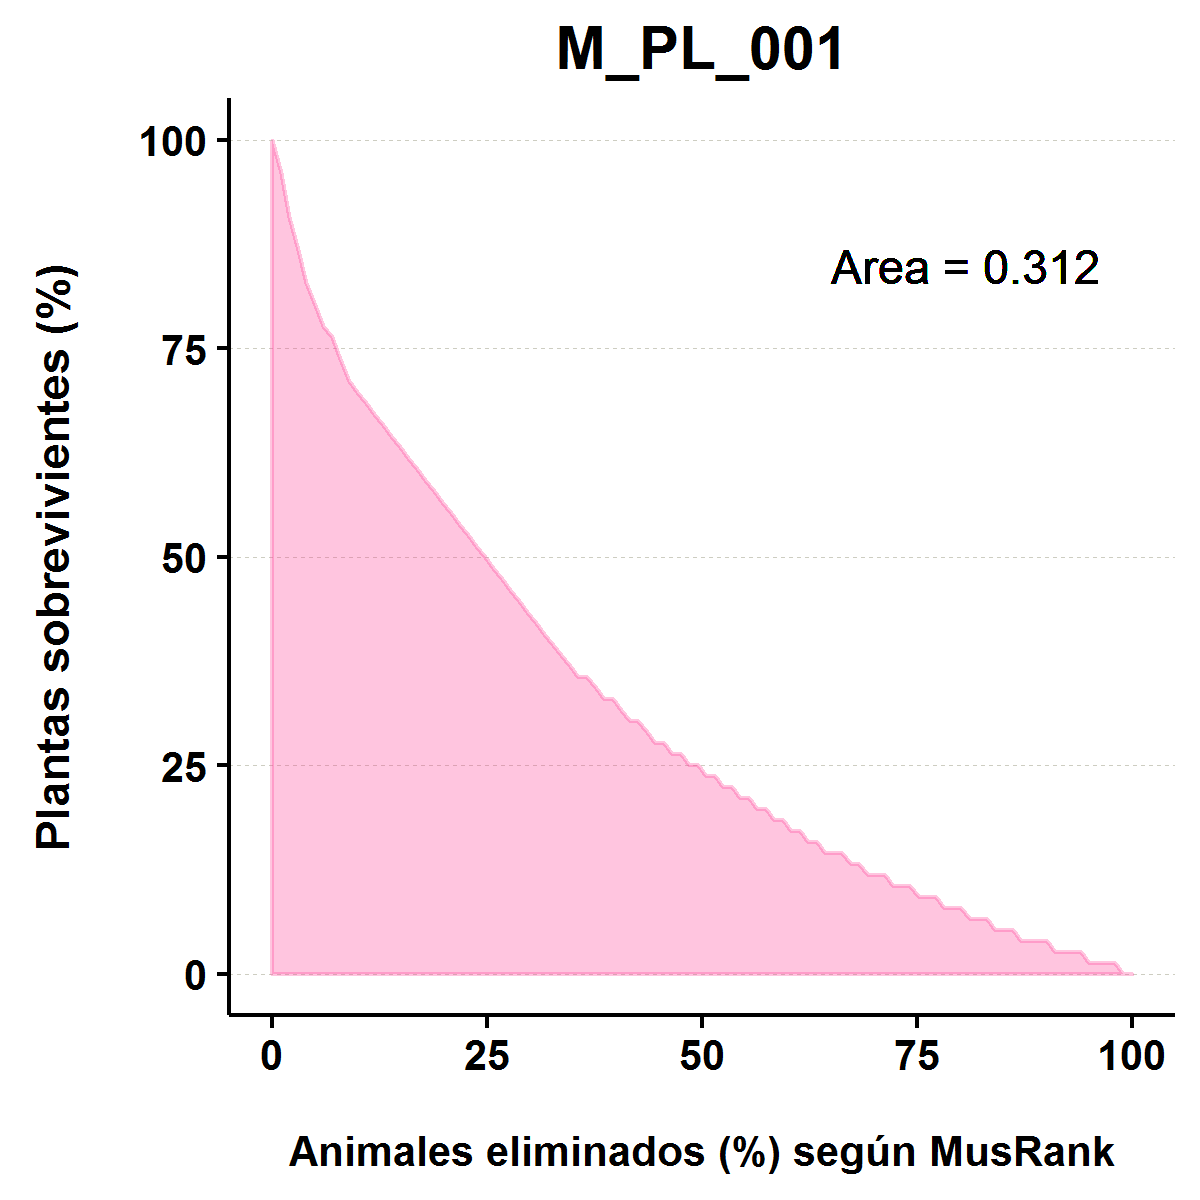
\includegraphics[scale=1]{Figures/DEST_M_PL_001_MRdunne_extinction_plot.png}
\caption{Curva de destrucción de la red de polinizadores $001$ ordenada por $MusRank$ y midiendo la fracción de plantas sobreviviente. El área normalizada bajo la curva es 0.312 (tabla \ref{table:dunne_destruction}).}
\label{fig:DEST_M_PL_001_MRdunne_extinction_plot}
\end{figure}

\section{Resultados}

El efecto de la extinción de un pequeño porcentaje de especies muy centrales puede resultar dramático para la comunidad, como muestra la figura \ref{fig:DEST_M_PL_012_ziggurat_hf_destruction}. Se han retirado tan solo $7$ especies de las $81$ originales, empleando como criterio de ordenación ${k}_{risk}$. La red queda reducida a menos de la mitad de su tamaño. La estructura interna se degrada de manera evidente, el núcleo central es una $2$-$shell$ y hay numerosas especies en la $1$-$shell$ muy expuestas. Por ejemplo, la desaparición de la especie de planta número $4$ con esta configuración arrastraría a $8$ especies adicionales.

\begin{figure}[htp!]
\centering
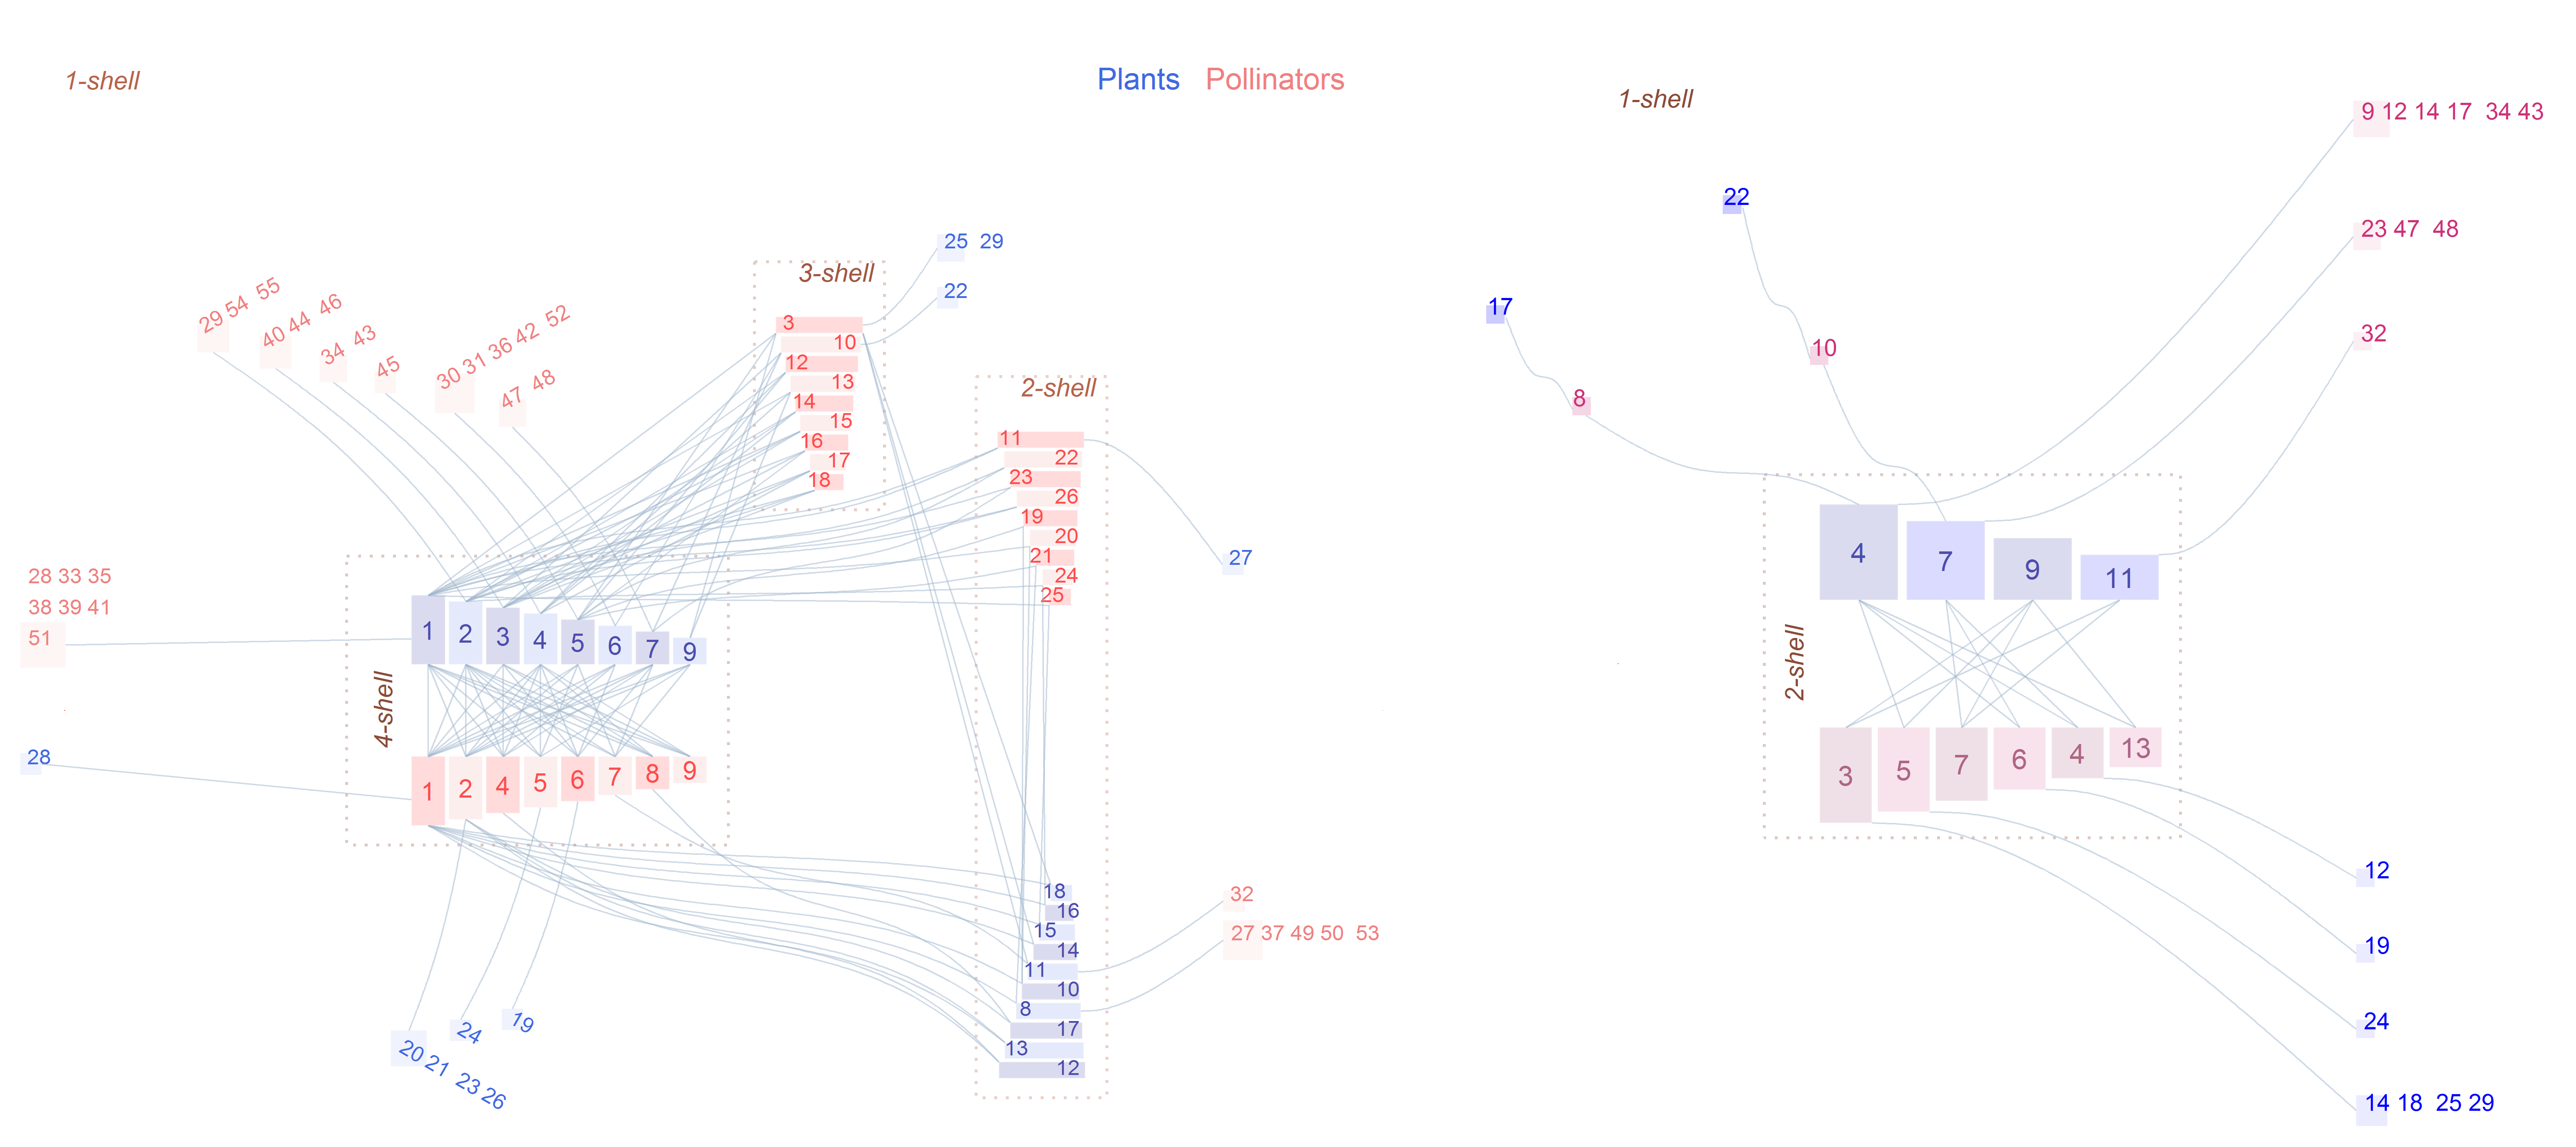
\includegraphics[scale=0.12]{Figures/DEST_M_PL_012_ziggurat_hf_destruction.png}
\caption {Destrucción de la componente gigante de la red de polinizadores número $012$ (Olesen, no publicada), ordenando por $k_{risk}$. Red original con $84$ especies (a). Componente gigante que queda tras retirar las $7$ especies más importantes, siguiendo esta secuencia: $planta1$, $planta2$, $polinizador2$, $polinizador1$, $planta3$, $planta6$ y $planta5$ (b).}
\label{fig:DEST_M_PL_012_ziggurat_hf_destruction}
\end{figure}

En la tabla \ref{table:DEST_halfgc_destruction} se han recogido los resultados del primer procedimiento de destrucción, medido en número de especies que hay que eliminar de la red, siguiendo el orden del criterio especificado para destruir la mitad de la componente gigante.

Según estos datos, $k_{risk}$ es el criterio más destructivo y por tanto el más eficaz para $76$ de las $89$ redes $(85.39\%)$; $k_{degree}$ para $44$, $(49.44\%)$; $degree$ para $58$, $(65.17\%)$ y
$eigenvector$ $centrality$ es el mejor para $29$ redes $(32.58\%)$. En numerosas ocasiones, sobre todo si la red es pequeña, varios índices pueden producir el
resultado óptimo, por eso la suma no es el $100\%$.

En la figura \ref{fig:DEST_krisk_kdegree_comparison_ES}a se comparan los rendimientos de los dos índices más eficaces. Se aprecia que ${k}_{risk}$ funciona de manera óptima cuando la destrucción se logra retirando un pequeño porcentaje de especies.

\clearpage
\begin{figure}[h!]
\centering
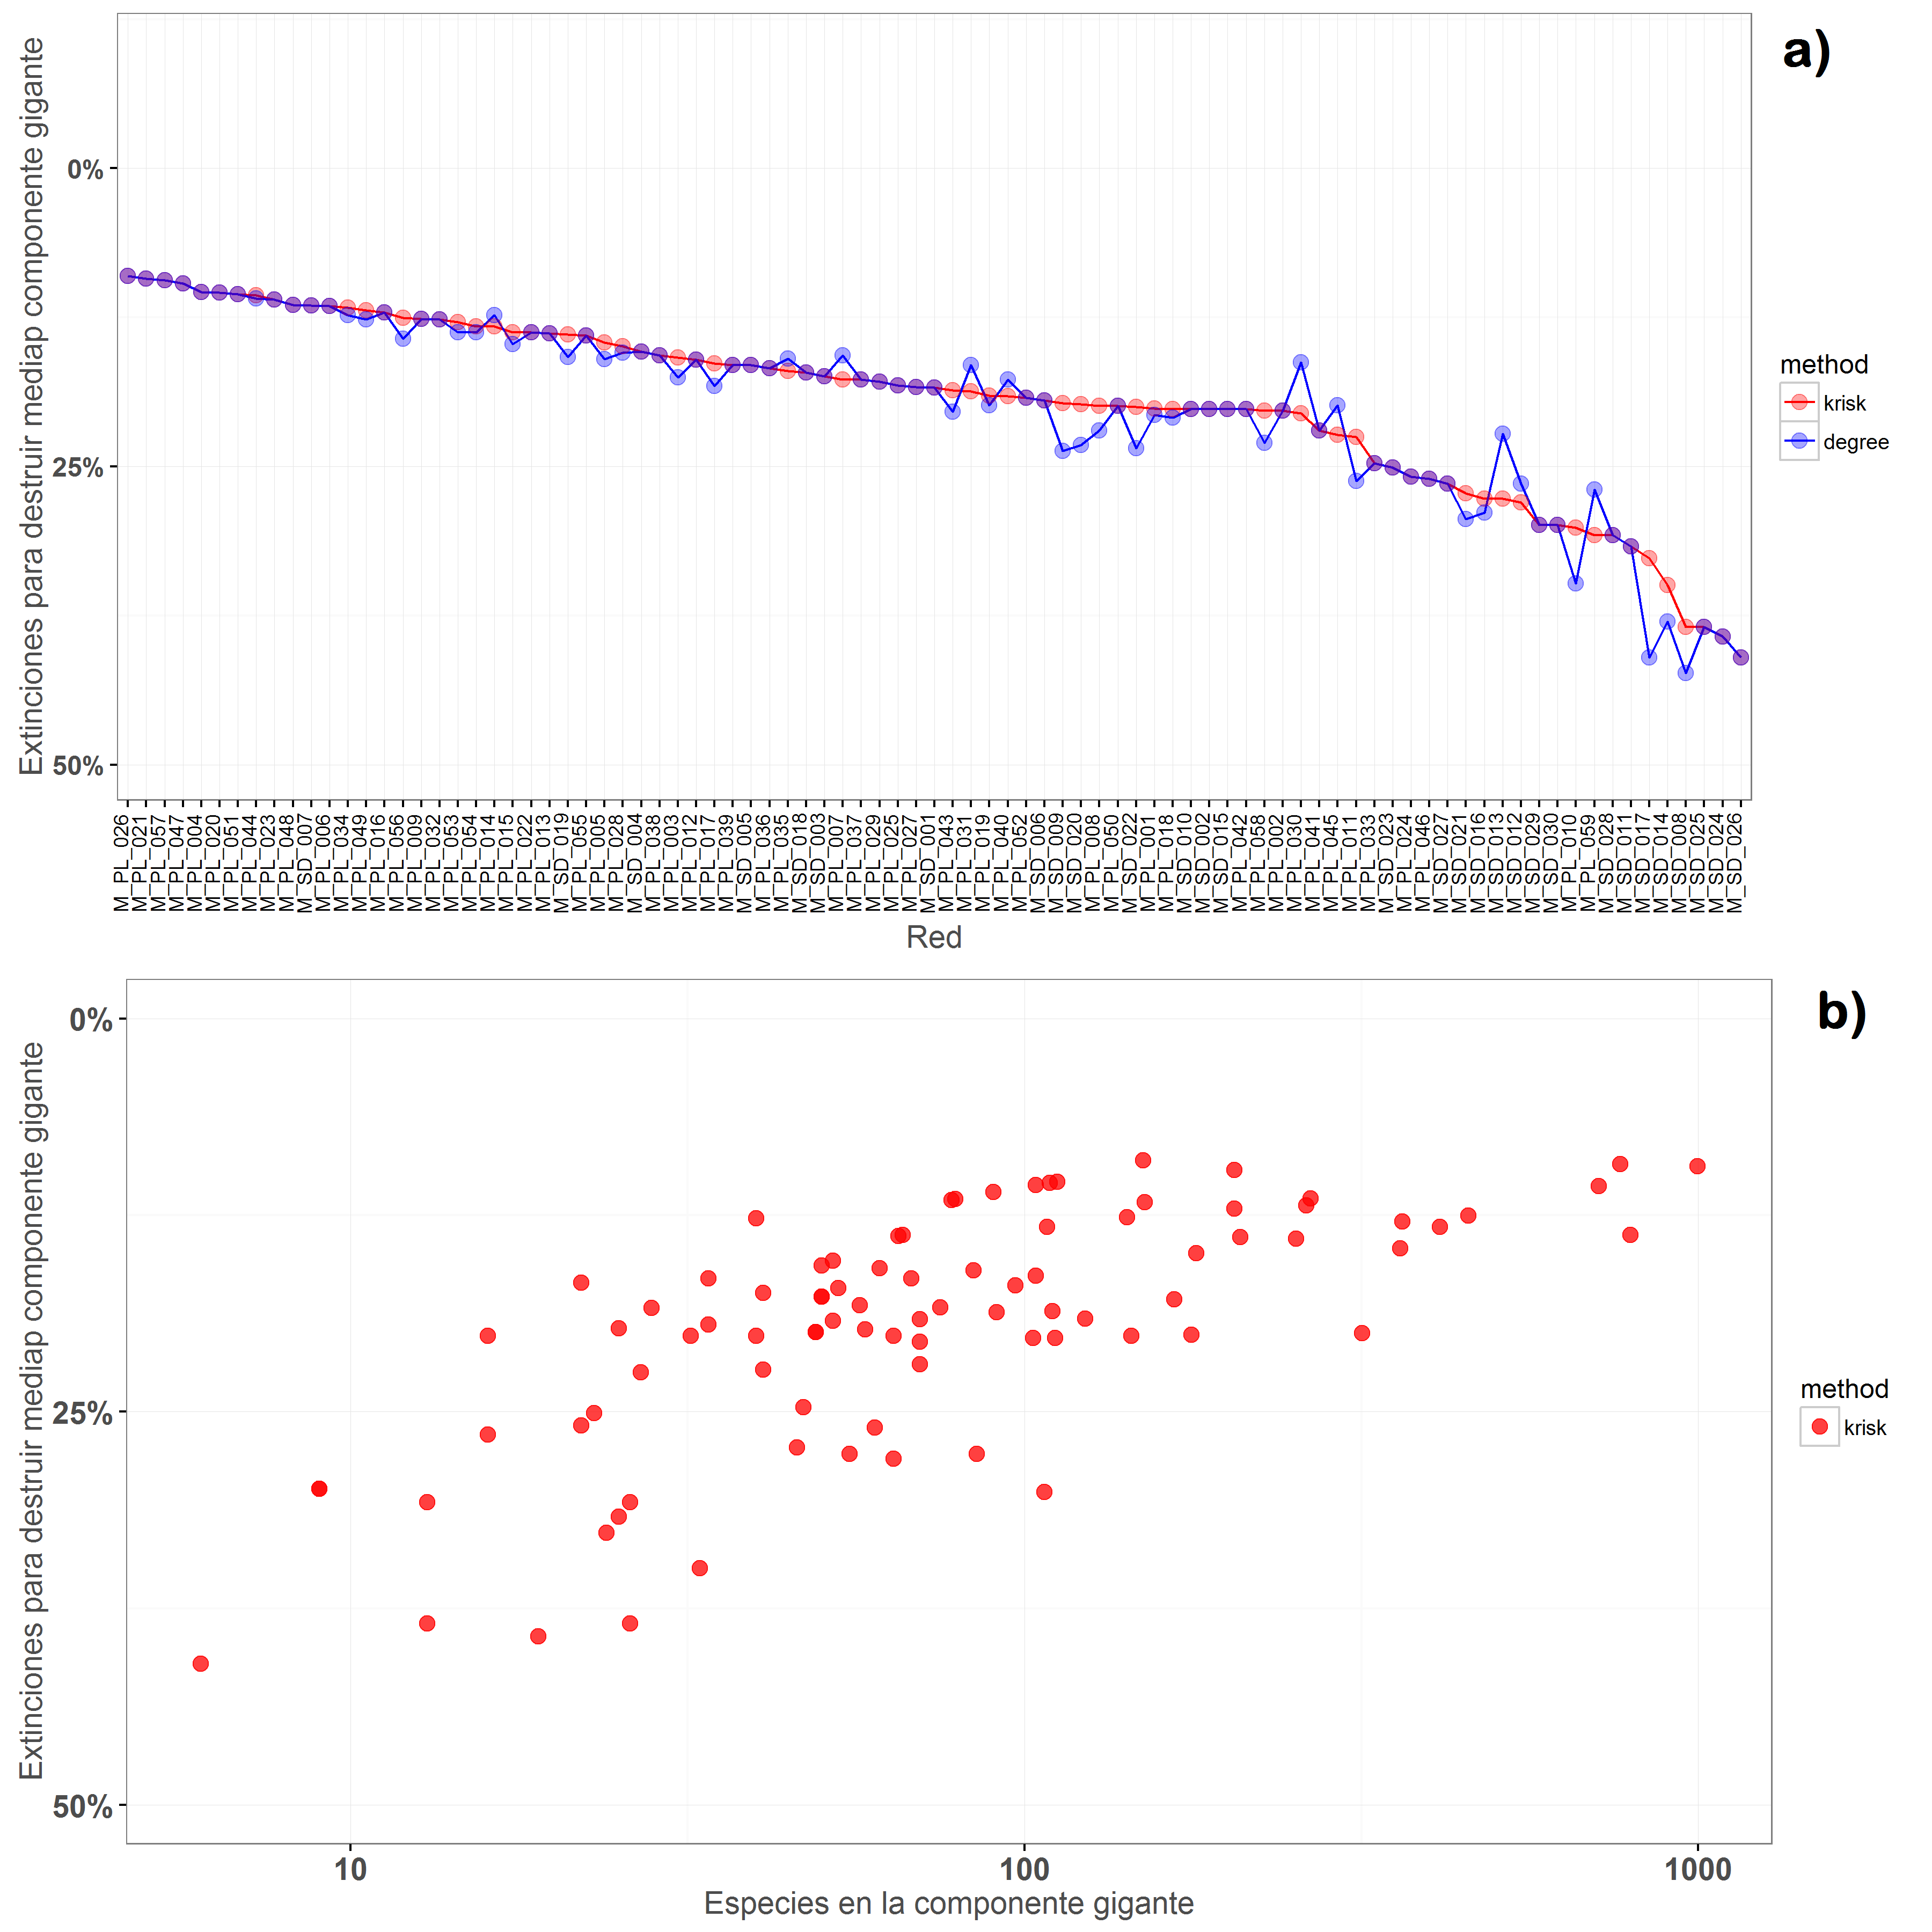
\includegraphics[scale=0.55]{Figures/DEST_krisk_kdegree_comparison_ES.png}
\caption {Comparación del rendimiento de los dos criterios más destructivos de la mitad de la componente gigante, $k_{risk}$ y $degree$ (a) y comportamiento de ${k}_{risk}$ en función del tamaño de la red (b).}
\label{fig:DEST_krisk_kdegree_comparison_ES}
\end{figure}

En la figura \ref{fig:DEST_krisk_kdegree_comparison_ES}b se ha representado el porcentaje de extinciones primarias que provoca la destrucción de la mitad de la componente gigante en función del tamaño de la red, usando ${k}_{risk}$. Para las redes muy pequeñas el porcentaje es grande, y se reduce de forma log lineal hasta llegar a las $100$ especies. A partir de ese punto, el porcentaje se estabiliza en torno al $12\%$. La gráfica es similar si en lugar de ${k}_{risk}$ se emplea otro criterio.

Los resultados del segundo método de destrucción (extinción solo de especies animales) se recogen en las tablas \ref{table:dunne_destruction} y \ref{table:juanma_destruction}. En la primera se tiene en cuenta la fracción de especies vegetales sobrevivientes y en la segunda la de la componente gigante que queda. Se mide el área bajo la curva de extinción; cuanto menor es, más destructivo es el criterio de ordenación.

\begin{figure}[h!]
\centering
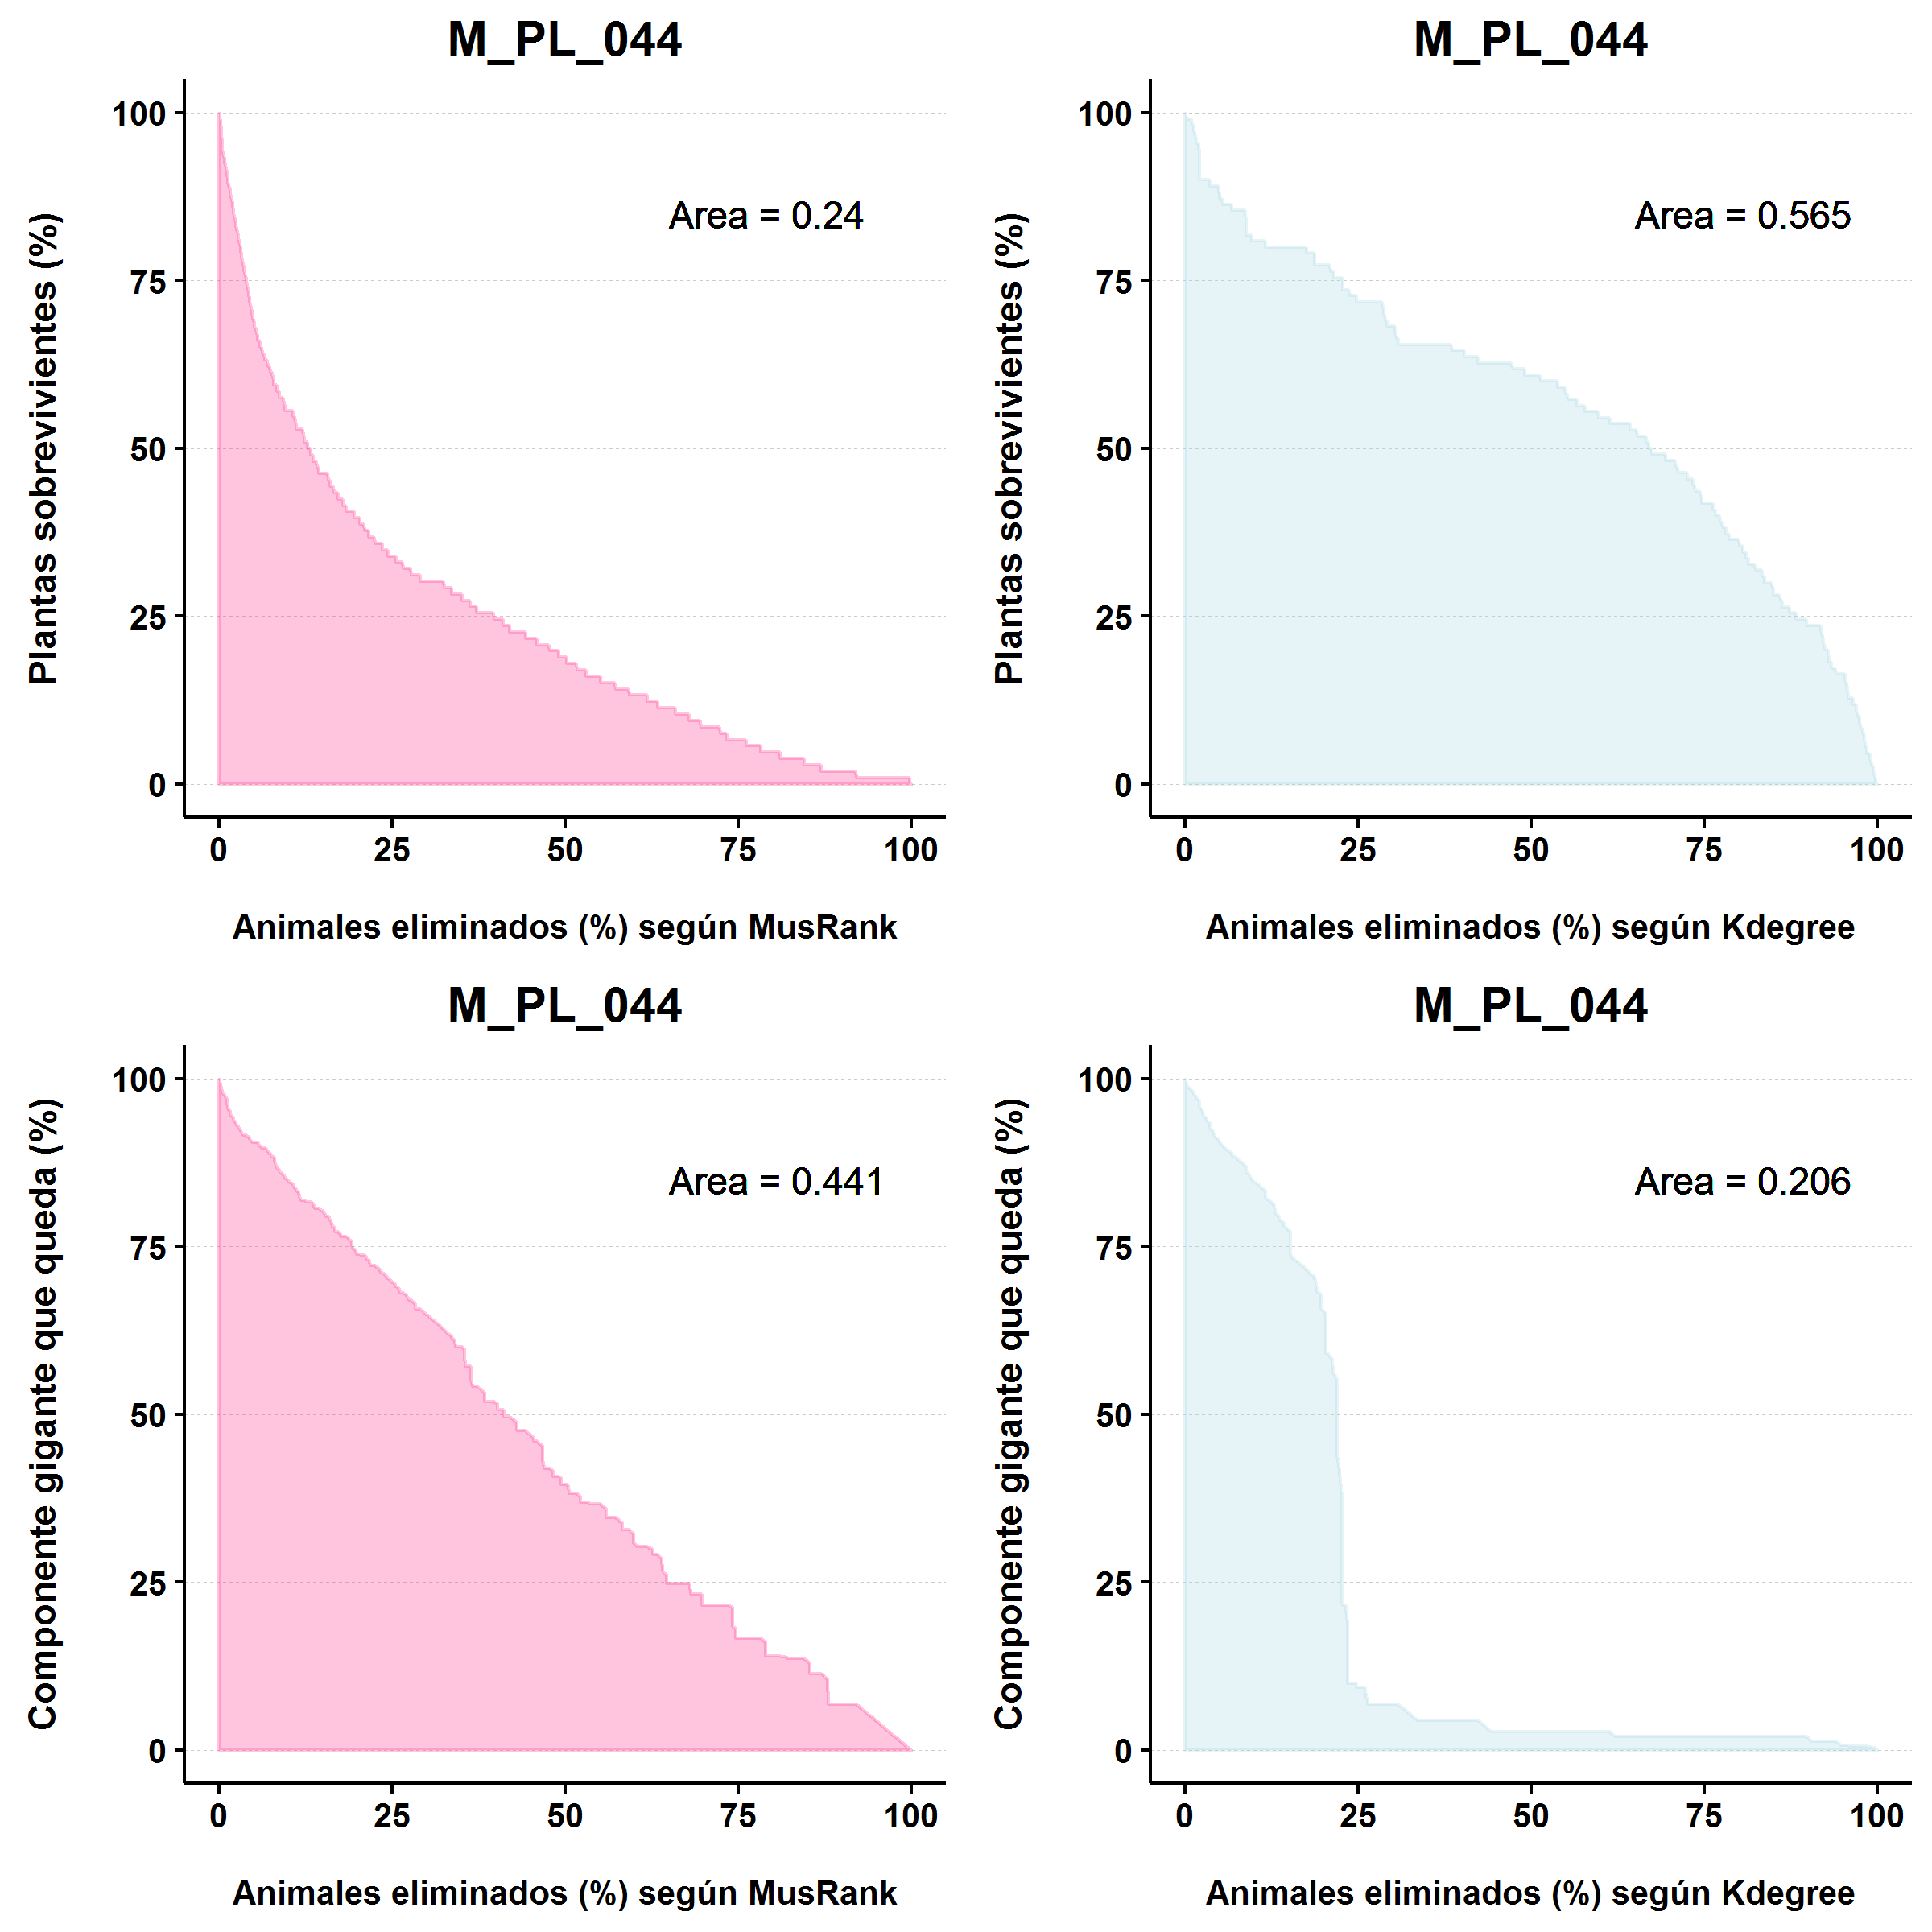
\includegraphics[scale=0.55]{Figures/DEST_M_PL_044_juanmamethod_extinction_plot.png}
\caption {Rendimiento del procedimiento de extinción de especies animales para $MusRank$ y ${k}_{degree}$ para las dos magnitudes de salida.}
\label{fig:DEST_M_PL_044_juanmamethod_extinction_plot}
\end{figure}

A primera vista, los resultados son paradójicos. Midiendo la fracción superviviente de especies vegetales, $MusRank$ es el mejor índice de destrucción para $89$ redes $(100\%)$; $k_{risk}$ para $7$, $(7.87\%)$; $k_{degree}$ para $8$, $(8.99\%)$; $degree$ para $8$, $(8.99\%)$ y $eigenvector$ $centrality$ el mejor para $8$ redes $(8.99\%)$. El comportamiento óptimo de $MusRank$ es el esperado, y está de acuerdo con lo publicado por \cite{dominguez2015ranking}. Hay que tener en cuenta que es un índice que se elabora partiendo de la naturaleza bipartita de la red y que este procedimiento mide los efectos de la perturbación sobre una clase en la contraria. El resto de índices, incluyendo las \textit{k magnitudes}, miden propiedades generales de la red.

Realizando la misma secuencia de extinciones primarias pero midiendo la fracción de componente gigante que queda, el rendimiento es muy diferente. $MusRank$ es el mejor solo para $18$ redes $(20.22\%)$; $k_{risk}$ para $39$, $(43.82\%)$; $k_{degree}$ para $58$, $(65.17\%)$; $degree$ para $44$, $(49.44\%)$ y $eigenvector$ $centrality$ para $23$ redes $(25.84\%)$. Los índices basados en \textit{k magnitudes} pasan a ser óptimos y $MusRank$ a la última posición.

La diferencia resulta tan notable (figura \ref{fig:DEST_M_PL_044_juanmamethod_extinction_plot}) que llevó a pensar en errores en el \textit{software} o en el método. Sin embargo, se han comprobado meticulosamente los datos intermedios y las secuencias de extinción, repitiéndose los resultados. La explicación tiene que ver con la naturaleza de los índices que se acaba de exponer. Al medir la fracción de componente gigante, resultan más destructivos los que ordenan todas las especies de la red por un mismo criterio y en este caso $MusRank$ es el único que difiere.

Para comprender la diferencia, el diagrama de zigurat resulta de gran ayuda.

\begin{figure}[h!]
\centering
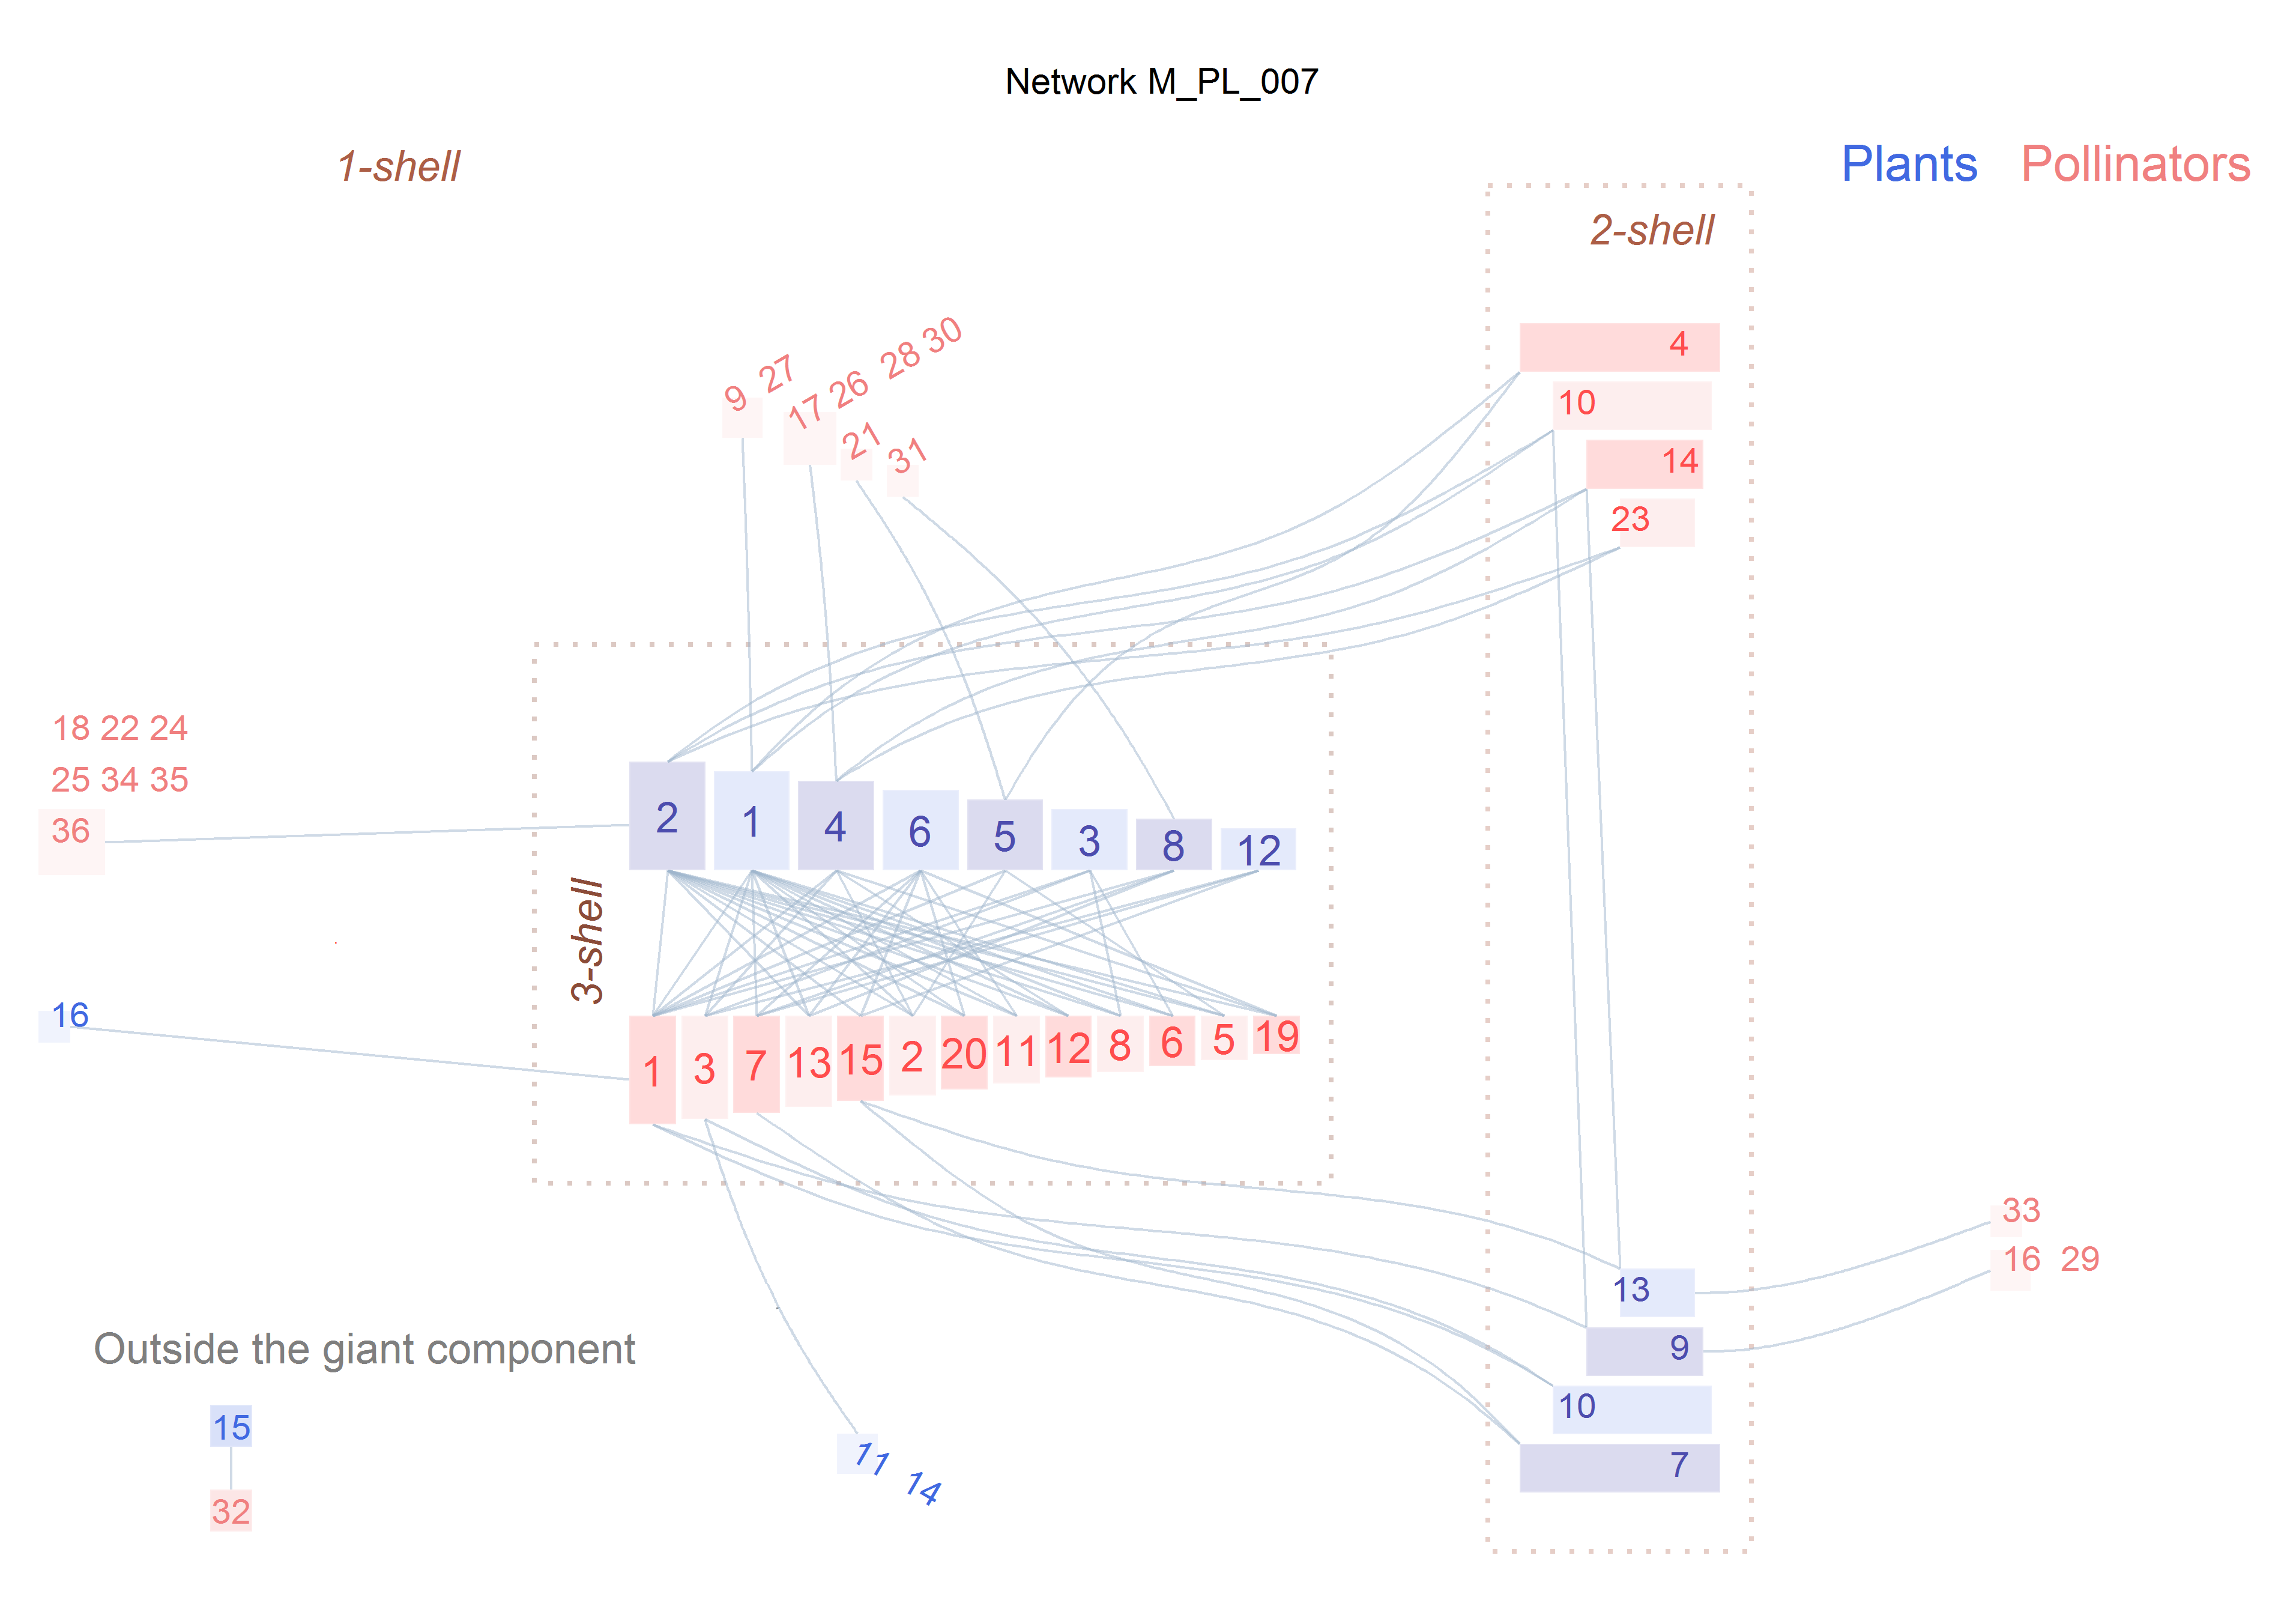
\includegraphics[scale=0.45]{Figures/DEST_M_PL_007_ziggurat.png}
\caption {Red de polinizadores en Shelfanger, Norfolk, Reino Unido \cite{dicks2002compartmentalization}.}
\label{fig:DEST_M_PL_007_ziggurat.png}
\end{figure}

La figura \ref{fig:DEST_M_PL_007_ziggurat.png} es una red de $36$ especies de planta y $16$ de polinizadores. Dos de ellas se encuentran desconectadas de la componente gigante por lo que el tamaño original de esta es $50$. Se provocan $10$ extinciones primarias, siguiendo dos criterios, ${k}_{degree}$ y $MusRank$. En el gráfico \ref{fig:DEST_destruccion_PL007.png} se ven los resultados. Mientras que $MusRank$ produce más extinciones de plantas, ${k}_{degree}$ reduce más el tamaño de la componente gigante. Además, la estructura de la red resultante con ${k}_{degree}$ es más frágil, con una \textit{shell} máxima $2$. La red que queda con $MusRank$ muestra una estructura más compleja y un núcleo central mejor conectado.

Este ejemplo explica la paradoja de cómo un mismo criterio puede resultar óptimo o mediocre en función de lo que se mida y esto tiene repercusiones prácticas. Si la política de conservación busca mantener la biodiversidad vegetal, $MusRank$  identifica mejor en qué especies de polinizadores deben
centrarse los esfuerzos. Si, por el contrario, lo que se pretende es conservar la comunidad en su conjunto, ${k}_{degree}$ señala las especies capitales, sin importar la clase a la que pertenecen.

\begin{figure}[htp!]
\centering
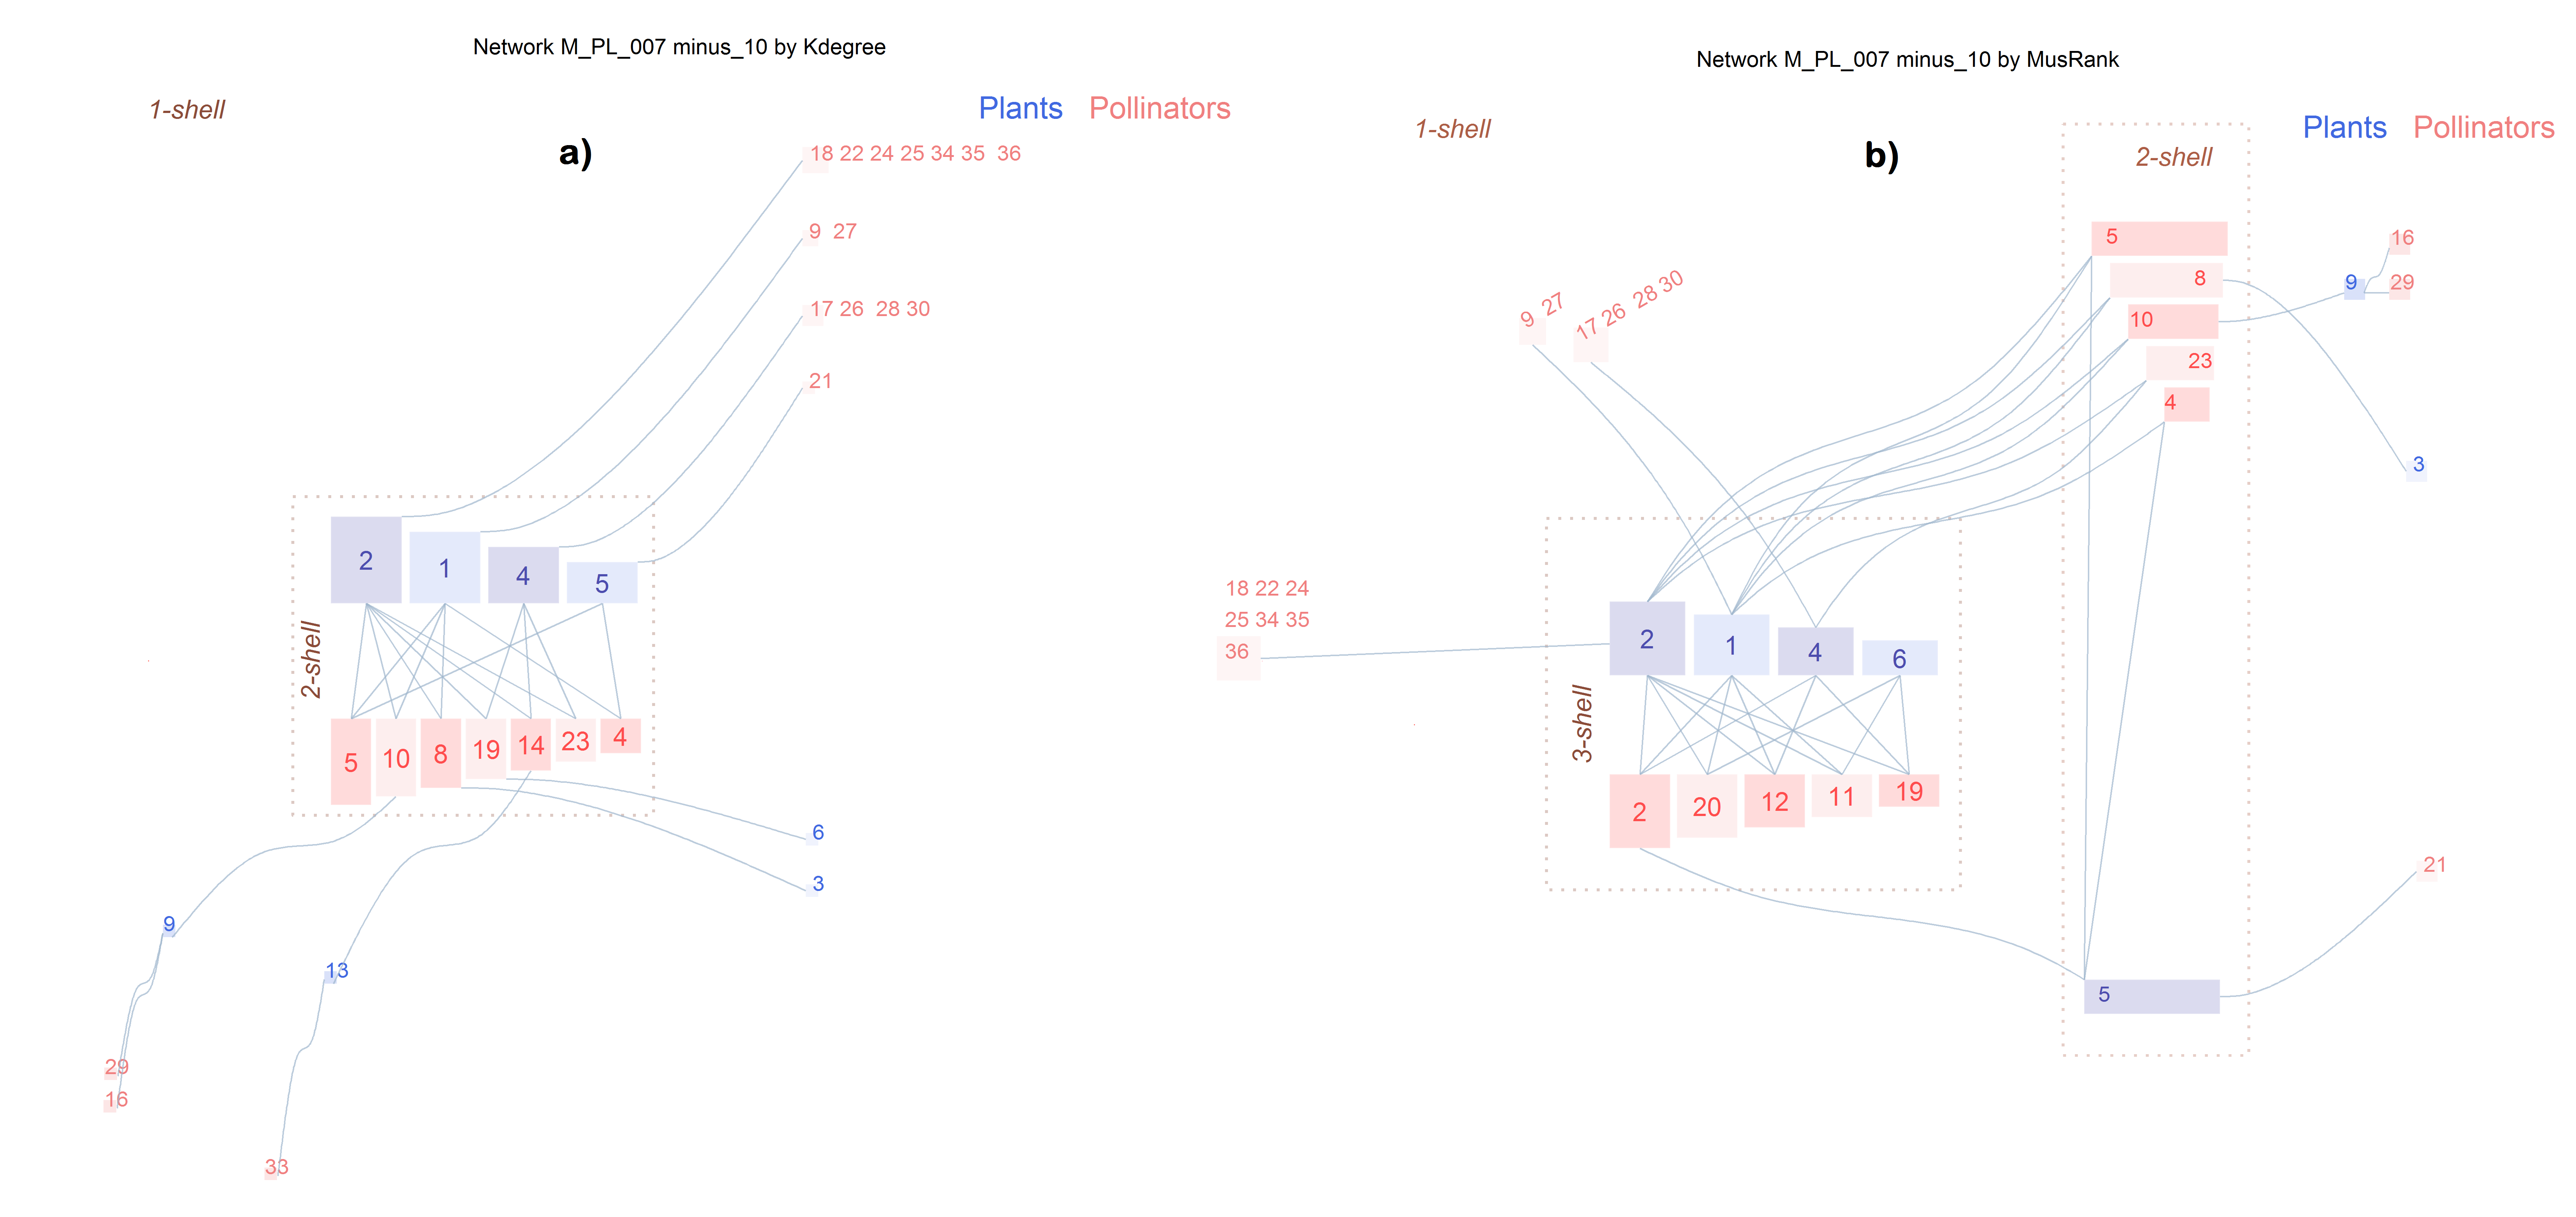
\includegraphics[scale=0.07]{Figures/DEST_destruccion_PL007.png}
\caption {Resultado de la retirada de $10$ especies animales de la red $M\_PL\_007$. Siguiendo el orden indicado por ${k}_{degree}$ (a). La componente gigante que queda tiene $32$ especies ($8$ de plantas, $24$ de polinizadores. Siguiendo $MusRank$ (b). La componente gigante tiene $33$ especies ($7$ de plantas, $26$ de polinizadores).}
\label{fig:DEST_destruccion_PL007.png}
\end{figure}

\section{Anexo: Videos}
\label{DES_ANEXO_videos}

Para presentar de una manera más visual los procesos de destrucción de redes, se han producido dos vídeos. En el primero de ellos se muestra la destrucción de la mitad de la componente gigante de la red $M\_PL\_050$. Comienza teniendo $49$ especies y queda reducida a $22$ con tan solo $6$ extinciones primarias. Puede verse en \url{https://www.youtube.com/watch?v=nvoWhLhjXks}.

En el segundo video se destruye la red $M\_PL\_007$ provocando extinciones primarias solo en las especies animales. Puede comprobarse el distinto estado final que se alcanza si se usan $MusRank$ y ${k}_{degree}$ como criterios de ordenación. Si se toma el primero, la red final tiene menos especies vegetales ($7$) que usando ${k}_{degree}$ ($8$). Sin embargo, el tamaño de la componente gigante que queda ($33$ especies) es mayor que con el segundo criterio ($32$). Puede verse en \url{https://www.youtube.com/watch?v=H1UxAClqCxg}. 

%\section{Conclusiones}
%
%La resistencia de las redes mutualistas es una cuestión de gran importancia para la conservación de la biovidersidad. La definición del término resistencia no es neutral, hemos comprobado como conduce a resultados aparentemente contradictorios.
%
%El índice ${k}_{risk}$ es el mejor para identificar qué especies pueden producir una degradación más rápida de la red. Un pequeño porcentaje de extinciones, en torno al $12\%$ para redes de más de $100$ especies, reduce el tamaño de la componente gigante a menos de la mitad.  
%
%Si se mide el proceso de destrucción completa, el resultado depende de la magnitud resultante elegida. El índice $MusRank$ es el más eficaz para identifcar las especies animales clave cuando se mide el porcentaje de especies vegetales supervivientes. Por el contrario, ${k}_{degree}$ es más conveniente para mantener la componente gigante.
%
%La variedad de índices es útil para el establecimiento de políticas de conservación. Dependiendo de los objetivos fijados los responsables podrán elegir el más adecuado.
\clearpage
\section{Anexo: Resultados de los procesos de destrucción}
\label{DES_ANEXO_halfgc}

\begin{table}[htbp]
\fontsize{2.3mm}{2.3mm}\selectfont
  \centering
      \caption{\label{table:DEST_halfgc_destruction} Número de especies que hay que eliminar de la red, siguiendo el orden del criterio especificado para destruir la mitad de la componente gigante. $k_{risk}$ es el mejor $76$ redes $(85.39\%)$; $k_{degree}$ para $44$, $(49.44\%)$; $degree$ para $58$, $(65.17\%)$ y
$eigenvector$ $centrality$ es el mejor para $29$ redes $(32.58\%)$.}

  %\begin{adjustbox}{angle=90}
    \begin{tabular}{lrrrrrrrrrrrr}
    \toprule
    $Network$ & $GC$ & $k_{risk}$ & $degree$ & $k_{degree}$ & $eigenv$ &    &$Network$ & $GC$ & $k_{risk}$ & $degree$ & $k_{degree}$ & $eigenv$ \\
    \midrule
        M\_PL\_001 & 177  & 22   & 23   & 22   & 23   &      & M\_PL\_046 & 60   & 11   & 11   & 13   & 14 \\
    M\_PL\_002 & 103  & 13   & 13   & 13   & 15   &      & M\_PL\_047 & 205  & 4    & 4    & 4    & 4 \\
    M\_PL\_003 & 61   & 5    & 6    & 6    & 6    &      & M\_PL\_048 & 266  & 10   & 10   & 9    & 12 \\
    M\_PL\_004 & 112  & 3    & 3    & 3    & 3    &      & M\_PL\_049 & 262  & 11   & 13   & 15   & 16 \\
    M\_PL\_005 & 361  & 25   & 30   & 36   & 42   &      & M\_PL\_050 & 49   & 6    & 6    & 7    & 7 \\
    M\_PL\_006 & 78   & 3    & 3    & 3    & 3    &      & M\_PL\_051 & 104  & 3    & 3    & 3    & 3 \\
    M\_PL\_007 & 50   & 5    & 4    & 4    & 4    &      & M\_PL\_052 & 52   & 6    & 6    & 6    & 7 \\
    M\_PL\_008 & 49   & 6    & 7    & 7    & 11   &      & M\_PL\_053 & 364  & 19   & 22   & 23   & 34 \\
    M\_PL\_009 & 142  & 7    & 7    & 8    & 12   &      & M\_PL\_054 & 414  & 23   & 25   & 27   & 30 \\
    M\_PL\_010 & 107  & 24   & 29   & 29   & 32   &      & M\_PL\_055 & 253  & 16   & 16   & 17   & 19 \\
    M\_PL\_011 & 27   & 4    & 5    & 6    & 6    &      & M\_PL\_056 & 456  & 22   & 30   & 33   & 43 \\
    M\_PL\_012 & 84   & 7    & 7    & 7    & 7    &      & M\_PL\_057 & 997  & 17   & 17   & 20   & 36 \\
    M\_PL\_013 & 65   & 4    & 4    & 4    & 5    &      & M\_PL\_058 & 111  & 14   & 17   & 19   & 20 \\
    M\_PL\_014 & 108  & 6    & 5    & 5    & 6    &      & M\_PL\_059 & 26   & 6    & 5    & 5    & 5 \\
    M\_PL\_015 & 793  & 48   & 56   & 60   & 87   &      & M\_SD\_001 & 28   & 3    & 3    & 3    & 5 \\
    M\_PL\_016 & 205  & 9    & 9    & 10   & 17   &      & M\_SD\_002 & 40   & 5    & 5    & 5    & 5 \\
    M\_PL\_017 & 104  & 9    & 11   & 11   & 11   &      & M\_SD\_003 & 41   & 4    & 4    & 4    & 4 \\
    M\_PL\_018 & 144  & 18   & 19   & 23   & 24   &      & M\_SD\_004 & 52   & 4    & 4    & 4    & 4 \\
    M\_PL\_019 & 123  & 14   & 15   & 16   & 18   &      & M\_SD\_005 & 34   & 3    & 3    & 3    & 3 \\
    M\_PL\_020 & 109  & 3    & 3    & 3    & 3    &      & M\_SD\_006 & 34   & 4    & 4    & 5    & 5 \\
    M\_PL\_021 & 766  & 12   & 12   & 12   & 38   &      & M\_SD\_007 & 79   & 3    & 3    & 3    & 3 \\
    M\_PL\_022 & 66   & 4    & 4    & 4    & 4    &      & M\_SD\_008 & 26   & 8    & 9    & 8    & 11 \\
    M\_PL\_023 & 90   & 3    & 3    & 3    & 3    &      & M\_SD\_009 & 25   & 3    & 4    & 4    & 5 \\
    M\_PL\_024 & 22   & 4    & 4    & 3    & 3    &      & M\_SD\_010 & 64   & 8    & 8    & 9    & 13 \\
    M\_PL\_025 & 57   & 6    & 6    & 6    & 10   &      & M\_SD\_011 & 25   & 6    & 6    & 5    & 6 \\
    M\_PL\_026 & 150  & 2    & 2    & 2    & 2    &      & M\_SD\_012 & 64   & 13   & 12   & 12   & 14 \\
    M\_PL\_027 & 75   & 8    & 8    & 9    & 11   &      & M\_SD\_013 & 55   & 11   & 8    & 19   & 14 \\
    M\_PL\_028 & 180  & 13   & 14   & 16   & 24   &      & M\_SD\_014 & 33   & 9    & 10   & 10   & 10 \\
    M\_PL\_029 & 167  & 17   & 17   & 17   & 19   &      & M\_SD\_015 & 32   & 4    & 4    & 4    & 4 \\
    M\_PL\_030 & 70   & 9    & 6    & 7    & 13   &      & M\_SD\_016 & 85   & 17   & 18   & 20   & 23 \\
    M\_PL\_031 & 91   & 10   & 8    & 13   & 17   &      & M\_SD\_017 & 24   & 6    & 8    & 10   & 10 \\
    M\_PL\_032 & 40   & 2    & 2    & 2    & 2    &      & M\_SD\_018 & 53   & 5    & 5    & 5    & 5 \\
    M\_PL\_033 & 47   & 8    & 8    & 10   & 12   &      & M\_SD\_019 & 209  & 13   & 17   & 20   & 21 \\
    M\_PL\_034 & 151  & 6    & 7    & 8    & 9    &      & M\_SD\_020 & 58   & 7    & 9    & 10   & 10 \\
    M\_PL\_035 & 97   & 9    & 8    & 9    & 9    &      & M\_SD\_021 & 46   & 9    & 10   & 10   & 10 \\
    M\_PL\_036 & 22   & 2    & 2    & 2    & 2    &      & M\_SD\_022 & 317  & 39   & 50   & 53   & 60 \\
    M\_PL\_037 & 50   & 5    & 5    & 5    & 7    &      & M\_SD\_023 & 23   & 4    & 4    & 4    & 4 \\
    M\_PL\_038 & 50   & 4    & 4    & 4    & 7    &      & M\_SD\_024 & 19   & 6    & 6    & 7    & 8 \\
    M\_PL\_039 & 68   & 6    & 6    & 9    & 10   &      & M\_SD\_025 & 13   & 4    & 4    & 4    & 4 \\
    M\_PL\_040 & 70   & 8    & 7    & 9    & 10   &      & M\_SD\_026 & 6    & 2    & 2    & 2    & 2 \\
    M\_PL\_041 & 70   & 10   & 10   & 11   & 12   &      & M\_SD\_027 & 16   & 3    & 3    & 3    & 3 \\
    M\_PL\_042 & 16   & 2    & 2    & 2    & 2    &      & M\_SD\_028 & 13   & 3    & 3    & 3    & 3 \\
    M\_PL\_043 & 110  & 12   & 14   & 14   & 19   &      & M\_SD\_029 & 9    & 2    & 2    & 2    & 2 \\
    M\_PL\_044 & 712  & 21   & 23   & 25   & 49   &      & M\_SD\_030 & 9    & 2    & 2    & 2    & 2 \\
    M\_PL\_045 & 41   & 6    & 5    & 7    & 8    &      &      &      &      &      &      &  \\
    \bottomrule
    \end{tabular}%
    %\end{adjustbox}

%[1] "krisk is the best for 76 networks (85.39%)"
%[1] "kdegree is the best for 44 networks (49.44%)"
%[1] "degree is the best for 58 networks (65.17%)"
%[1] "eigen is the best for 29 networks (32.58%)"
\end{table}%

\begin{table}[hp]
\fontsize{2.8mm}{2.8mm}\selectfont
  \centering
    \caption{\label{table:dunne_destruction} Áreas bajo las curvas normalizadas de destrucción, de acuerdo al índice de ordenación especificado, cuando la fracción de plantas supervivientes se representa en relación a la fracción de extinciones de animales. $MusRank$ es el mejor para $89$ redes $(100\%)$;
$k_{risk}$ el mejor para $7$, $(7.87\%)$; $k_{degree}$ para $8$, $(8.99\%)$; $degree$ para $8$, $(8.99\%)$ y
$eigenvector$ $centrality$ el mejor para $8$ redes $(8.99\%)$.}
    \begin{adjustbox}{angle=90}
    \begin{tabular}{lrrrrrrrrrrrr}
    \toprule
    $Network$ & $MR$ & $k_{risk}$ & $k_{degree}$ & $degree$ & $eigenv$ &    & $Network$ & $MR$ & $k_{risk}$ & $k_{degree}$ & $degree$ & $eigenv$ \\
    \midrule
       M\_PL\_001 & 0,312 & 0,42 & 0,411 & 0,394 & 0,42 &      & M\_PL\_046 & 0,658 & 0,736 & 0,753 & 0,754 & 0,736 \\
    M\_PL\_002 & 0,359 & 0,457 & 0,464 & 0,456 & 0,457 &      & M\_PL\_047 & 0,309 & 0,65 & 0,653 & 0,652 & 0,653 \\
    M\_PL\_003 & 0,29 & 0,331 & 0,307 & 0,321 & 0,331 &      & M\_PL\_048 & 0,334 & 0,638 & 0,659 & 0,651 & 0,639 \\
    M\_PL\_004 & 0,282 & 0,677 & 0,677 & 0,677 & 0,673 &      & M\_PL\_049 & 0,322 & 0,743 & 0,677 & 0,676 & 0,74 \\
    M\_PL\_005 & 0,276 & 0,509 & 0,52 & 0,502 & 0,508 &      & M\_PL\_050 & 0,398 & 0,576 & 0,506 & 0,5  & 0,593 \\
    M\_PL\_006 & 0,249 & 0,499 & 0,49 & 0,486 & 0,499 &      & M\_PL\_051 & 0,312 & 0,692 & 0,689 & 0,646 & 0,689 \\
    M\_PL\_007 & 0,329 & 0,52 & 0,492 & 0,486 & 0,522 &      & M\_PL\_052 & 0,412 & 0,659 & 0,657 & 0,656 & 0,656 \\
    M\_PL\_008 & 0,525 & 0,705 & 0,709 & 0,705 & 0,705 &      & M\_PL\_053 & 0,251 & 0,479 & 0,455 & 0,459 & 0,482 \\
    M\_PL\_009 & 0,358 & 0,67 & 0,628 & 0,615 & 0,669 &      & M\_PL\_054 & 0,257 & 0,544 & 0,512 & 0,505 & 0,544 \\
    M\_PL\_010 & 0,6  & 0,709 & 0,704 & 0,708 & 0,707 &      & M\_PL\_055 & 0,293 & 0,562 & 0,577 & 0,56 & 0,562 \\
    M\_PL\_011 & 0,388 & 0,399 & 0,399 & 0,399 & 0,399 &      & M\_PL\_056 & 0,27 & 0,534 & 0,549 & 0,531 & 0,534 \\
    M\_PL\_012 & 0,272 & 0,366 & 0,345 & 0,332 & 0,363 &      & M\_PL\_057 & 0,202 & 0,549 & 0,519 & 0,508 & 0,547 \\
    M\_PL\_013 & 0,435 & 0,821 & 0,821 & 0,821 & 0,812 &      & M\_PL\_058 & 0,417 & 0,541 & 0,558 & 0,555 & 0,54 \\
    M\_PL\_014 & 0,273 & 0,54 & 0,563 & 0,531 & 0,538 &      & M\_PL\_059 & 0,364 & 0,364 & 0,37 & 0,37 & 0,37 \\
    M\_PL\_015 & 0,379 & 0,668 & 0,657 & 0,654 & 0,667 &      & M\_SD\_001 & 0,459 & 0,514 & 0,514 & 0,514 & 0,507 \\
    M\_PL\_016 & 0,364 & 0,771 & 0,696 & 0,695 & 0,766 &      & M\_SD\_002 & 0,5  & 0,5  & 0,5  & 0,5  & 0,5 \\
    M\_PL\_017 & 0,37 & 0,513 & 0,519 & 0,503 & 0,513 &      & M\_SD\_003 & 0,305 & 0,326 & 0,317 & 0,317 & 0,326 \\
    M\_PL\_018 & 0,445 & 0,625 & 0,624 & 0,621 & 0,623 &      & M\_SD\_004 & 0,212 & 0,228 & 0,24 & 0,228 & 0,228 \\
    M\_PL\_019 & 0,347 & 0,56 & 0,537 & 0,54 & 0,56 &      & M\_SD\_005 & 0,266 & 0,39 & 0,353 & 0,266 & 0,397 \\
    M\_PL\_020 & 0,267 & 0,601 & 0,545 & 0,548 & 0,598 &      & M\_SD\_006 & 0,308 & 0,355 & 0,347 & 0,347 & 0,355 \\
    M\_PL\_021 & 0,176 & 0,499 & 0,506 & 0,467 & 0,498 &      & M\_SD\_007 & 0,253 & 0,253 & 0,253 & 0,253 & 0,253 \\
    M\_PL\_022 & 0,251 & 0,493 & 0,492 & 0,443 & 0,5  &      & M\_SD\_008 & 0,688 & 0,694 & 0,712 & 0,706 & 0,694 \\
    M\_PL\_023 & 0,229 & 0,727 & 0,704 & 0,535 & 0,726 &      & M\_SD\_009 & 0,417 & 0,528 & 0,528 & 0,528 & 0,528 \\
    M\_PL\_024 & 0,411 & 0,539 & 0,539 & 0,528 & 0,539 &      & M\_SD\_010 & 0,493 & 0,499 & 0,527 & 0,513 & 0,499 \\
    M\_PL\_025 & 0,434 & 0,622 & 0,662 & 0,604 & 0,622 &      & M\_SD\_011 & 0,529 & 0,586 & 0,542 & 0,542 & 0,586 \\
    M\_PL\_026 & 0,214 & 0,4  & 0,378 & 0,297 & 0,4  &      & M\_SD\_012 & 0,391 & 0,412 & 0,432 & 0,434 & 0,412 \\
    M\_PL\_027 & 0,447 & 0,591 & 0,609 & 0,601 & 0,589 &      & M\_SD\_013 & 0,483 & 0,563 & 0,675 & 0,598 & 0,563 \\
    M\_PL\_028 & 0,327 & 0,625 & 0,619 & 0,594 & 0,625 &      & M\_SD\_014 & 0,522 & 0,529 & 0,54 & 0,54 & 0,529 \\
    M\_PL\_029 & 0,311 & 0,506 & 0,488 & 0,484 & 0,511 &      & M\_SD\_015 & 0,744 & 0,848 & 0,848 & 0,848 & 0,856 \\
    M\_PL\_030 & 0,395 & 0,614 & 0,605 & 0,591 & 0,613 &      & M\_SD\_016 & 0,632 & 0,693 & 0,682 & 0,68 & 0,693 \\
    M\_PL\_031 & 0,331 & 0,384 & 0,386 & 0,381 & 0,384 &      & M\_SD\_017 & 0,641 & 0,672 & 0,688 & 0,672 & 0,672 \\
    M\_PL\_032 & 0,389 & 0,565 & 0,634 & 0,582 & 0,535 &      & M\_SD\_018 & 0,341 & 0,537 & 0,481 & 0,463 & 0,537 \\
    M\_PL\_033 & 0,664 & 0,669 & 0,675 & 0,675 & 0,669 &      & M\_SD\_019 & 0,319 & 0,344 & 0,36 & 0,357 & 0,344 \\
    M\_PL\_034 & 0,25 & 0,44 & 0,432 & 0,425 & 0,447 &      & M\_SD\_020 & 0,316 & 0,343 & 0,363 & 0,35 & 0,343 \\
    M\_PL\_035 & 0,312 & 0,375 & 0,389 & 0,369 & 0,375 &      & M\_SD\_021 & 0,425 & 0,463 & 0,472 & 0,463 & 0,463 \\
    M\_PL\_036 & 0,431 & 0,458 & 0,467 & 0,467 & 0,458 &      & M\_SD\_022 & 0,352 & 0,375 & 0,389 & 0,383 & 0,375 \\
    M\_PL\_037 & 0,515 & 0,628 & 0,635 & 0,635 & 0,62 &      & M\_SD\_023 & 0,388 & 0,4  & 0,388 & 0,388 & 0,4 \\
    M\_PL\_038 & 0,47 & 0,688 & 0,69 & 0,688 & 0,679 &      & M\_SD\_024 & 0,513 & 0,526 & 0,536 & 0,536 & 0,526 \\
    M\_PL\_039 & 0,345 & 0,508 & 0,497 & 0,499 & 0,5  &      & M\_SD\_025 & 0,472 & 0,556 & 0,556 & 0,556 & 0,556 \\
    M\_PL\_040 & 0,294 & 0,475 & 0,47 & 0,428 & 0,475 &      & M\_SD\_026 & 0,333 & 0,333 & 0,333 & 0,333 & 0,333 \\
    M\_PL\_041 & 0,398 & 0,543 & 0,556 & 0,536 & 0,543 &      & M\_SD\_027 & 0,475 & 0,475 & 0,475 & 0,475 & 0,475 \\
    M\_PL\_042 & 0,345 & 0,369 & 0,369 & 0,369 & 0,369 &      & M\_SD\_028 & 0,443 & 0,443 & 0,443 & 0,443 & 0,443 \\
    M\_PL\_043 & 0,441 & 0,626 & 0,61 & 0,611 & 0,626 &      & M\_SD\_029 & 0,5  & 0,5  & 0,5  & 0,5  & 0,5 \\
    M\_PL\_044 & 0,24 & 0,574 & 0,566 & 0,551 & 0,574 &      & M\_SD\_030 & 0,458 & 0,458 & 0,458 & 0,458 & 0,458 \\
    M\_PL\_045 & 0,332 & 0,375 & 0,401 & 0,392 & 0,375 &      &      &      &      &      &      &  \\
    \bottomrule
    \end{tabular}%
    \end{adjustbox}
%[1] "Juanma code with dunnemethod"
%[1] "krisk is the best for 7 networks (7.87%)"
%[1] "kdegree is the best for 8 networks (8.99%)"
%[1] "degree is the best for 8 networks (8.99%)"
%[1] "MusRank is the best for 89 networks (100.00%)"
%[1] "eigenc is the best for 8 networks (8.99%)"
\end{table}%

\clearpage
% Table generated by Excel2LaTeX from sheet 'zscores_all'
\begin{table}[htbp]
\fontsize{2.8mm}{2.8mm}\selectfont
  \centering
    \caption{\label{table:juanma_destruction} Áreas bajo las curvas normalizadas de destrucción, de acuerdo al índice de ordenación especificado, cuando la fracción de la componente gigante superviviente se representa en relación a la fracción de extinciones de animales. $MusRank$ es el mejor para $18$ redes $(20.22\%)$;
$k_{risk}$ para $39$, $(43.82\%)$; $k_{degree}$ para $58$, $(65.17\%)$; $degree$ para $44$, $(49.44\%)$ y
$eigenvector$ $centrality$ es el mejor para $23$ redes $(25.84\%)$.}

   \begin{adjustbox}{angle=90}
    \begin{tabular}{lrrrrrrrrrrrr}
    \toprule
    $Network$ & $MR$ & $k_{risk}$ & $k_{degree}$ & $degree$ & $eigenv$ &    & $Network$ & $MR$ & $k_{risk}$ & $k_{degree}$ & $degree$ & $eigenv$ \\
    \midrule
    M\_PL\_001 & 0,316 & 0,253 & 0,221 & 0,222 & 0,255 &      & M\_PL\_046 & 0,506 & 0,497 & 0,501 & 0,501 & 0,499 \\
    M\_PL\_002 & 0,434 & 0,348 & 0,324 & 0,323 & 0,32 &      & M\_PL\_047 & 0,463 & 0,37 & 0,369 & 0,37 & 0,362 \\
    M\_PL\_003 & 0,218 & 0,204 & 0,21 & 0,207 & 0,215 &      & M\_PL\_048 & 0,472 & 0,39 & 0,392 & 0,39 & 0,4 \\
    M\_PL\_004 & 0,466 & 0,37 & 0,37 & 0,37 & 0,384 &      & M\_PL\_049 & 0,466 & 0,337 & 0,328 & 0,327 & 0,396 \\
    M\_PL\_005 & 0,438 & 0,315 & 0,293 & 0,29 & 0,348 &      & M\_PL\_050 & 0,407 & 0,341 & 0,329 & 0,329 & 0,321 \\
    M\_PL\_006 & 0,437 & 0,39 & 0,393 & 0,392 & 0,393 &      & M\_PL\_051 & 0,438 & 0,335 & 0,334 & 0,335 & 0,376 \\
    M\_PL\_007 & 0,447 & 0,335 & 0,324 & 0,329 & 0,351 &      & M\_PL\_052 & 0,45 & 0,302 & 0,3  & 0,302 & 0,338 \\
    M\_PL\_008 & 0,479 & 0,446 & 0,437 & 0,446 & 0,439 &      & M\_PL\_053 & 0,405 & 0,235 & 0,205 & 0,21 & 0,215 \\
    M\_PL\_009 & 0,433 & 0,283 & 0,271 & 0,271 & 0,32 &      & M\_PL\_054 & 0,434 & 0,247 & 0,227 & 0,235 & 0,329 \\
    M\_PL\_010 & 0,509 & 0,489 & 0,479 & 0,48 & 0,497 &      & M\_PL\_055 & 0,444 & 0,311 & 0,245 & 0,234 & 0,356 \\
    M\_PL\_011 & 0,417 & 0,42 & 0,411 & 0,411 & 0,398 &      & M\_PL\_056 & 0,414 & 0,297 & 0,237 & 0,242 & 0,35 \\
    M\_PL\_012 & 0,345 & 0,294 & 0,302 & 0,284 & 0,317 &      & M\_PL\_057 & 0,46 & 0,33 & 0,25 & 0,232 & 0,336 \\
    M\_PL\_013 & 0,472 & 0,333 & 0,332 & 0,326 & 0,383 &      & M\_PL\_058 & 0,43 & 0,37 & 0,369 & 0,364 & 0,384 \\
    M\_PL\_014 & 0,438 & 0,368 & 0,368 & 0,373 & 0,468 &      & M\_PL\_059 & 0,408 & 0,395 & 0,398 & 0,398 & 0,395 \\
    M\_PL\_015 & 0,478 & 0,414 & 0,399 & 0,399 & 0,418 &      & M\_SD\_001 & 0,449 & 0,385 & 0,385 & 0,385 & 0,385 \\
    M\_PL\_016 & 0,469 & 0,326 & 0,323 & 0,325 & 0,395 &      & M\_SD\_002 & 0,49 & 0,49 & 0,49 & 0,49 & 0,49 \\
    M\_PL\_017 & 0,458 & 0,414 & 0,42 & 0,416 & 0,423 &      & M\_SD\_003 & 0,333 & 0,314 & 0,283 & 0,286 & 0,283 \\
    M\_PL\_018 & 0,45 & 0,348 & 0,343 & 0,342 & 0,358 &      & M\_SD\_004 & 0,251 & 0,233 & 0,23 & 0,233 & 0,245 \\
    M\_PL\_019 & 0,444 & 0,345 & 0,308 & 0,31 & 0,327 &      & M\_SD\_005 & 0,365 & 0,266 & 0,266 & 0,282 & 0,257 \\
    M\_PL\_020 & 0,443 & 0,345 & 0,342 & 0,343 & 0,389 &      & M\_SD\_006 & 0,344 & 0,305 & 0,305 & 0,305 & 0,302 \\
    M\_PL\_021 & 0,456 & 0,315 & 0,214 & 0,244 & 0,407 &      & M\_SD\_007 & 0,243 & 0,243 & 0,243 & 0,243 & 0,243 \\
    M\_PL\_022 & 0,418 & 0,309 & 0,288 & 0,289 & 0,386 &      & M\_SD\_008 & 0,606 & 0,61 & 0,622 & 0,618 & 0,626 \\
    M\_PL\_023 & 0,433 & 0,288 & 0,284 & 0,297 & 0,29 &      & M\_SD\_009 & 0,394 & 0,329 & 0,333 & 0,333 & 0,301 \\
    M\_PL\_024 & 0,503 & 0,328 & 0,328 & 0,294 & 0,339 &      & M\_SD\_010 & 0,488 & 0,493 & 0,515 & 0,504 & 0,519 \\
    M\_PL\_025 & 0,453 & 0,446 & 0,452 & 0,447 & 0,458 &      & M\_SD\_011 & 0,474 & 0,455 & 0,44 & 0,44 & 0,44 \\
    M\_PL\_026 & 0,324 & 0,209 & 0,216 & 0,221 & 0,197 &      & M\_SD\_012 & 0,36 & 0,328 & 0,357 & 0,344 & 0,361 \\
    M\_PL\_027 & 0,459 & 0,272 & 0,267 & 0,267 & 0,291 &      & M\_SD\_013 & 0,477 & 0,519 & 0,605 & 0,554 & 0,59 \\
    M\_PL\_028 & 0,444 & 0,378 & 0,349 & 0,335 & 0,374 &      & M\_SD\_014 & 0,498 & 0,502 & 0,507 & 0,507 & 0,507 \\
    M\_PL\_029 & 0,427 & 0,328 & 0,301 & 0,3  & 0,327 &      & M\_SD\_015 & 0,525 & 0,53 & 0,53 & 0,53 & 0,53 \\
    M\_PL\_030 & 0,466 & 0,27 & 0,251 & 0,263 & 0,348 &      & M\_SD\_016 & 0,495 & 0,484 & 0,485 & 0,485 & 0,485 \\
    M\_PL\_031 & 0,319 & 0,241 & 0,261 & 0,224 & 0,286 &      & M\_SD\_017 & 0,584 & 0,573 & 0,584 & 0,573 & 0,584 \\
    M\_PL\_032 & 0,432 & 0,367 & 0,378 & 0,37 & 0,395 &      & M\_SD\_018 & 0,411 & 0,21 & 0,168 & 0,175 & 0,223 \\
    M\_PL\_033 & 0,533 & 0,489 & 0,491 & 0,491 & 0,516 &      & M\_SD\_019 & 0,353 & 0,373 & 0,386 & 0,384 & 0,406 \\
    M\_PL\_034 & 0,449 & 0,363 & 0,361 & 0,359 & 0,366 &      & M\_SD\_020 & 0,413 & 0,413 & 0,422 & 0,416 & 0,423 \\
    M\_PL\_035 & 0,364 & 0,337 & 0,35 & 0,32 & 0,36 &      & M\_SD\_021 & 0,459 & 0,459 & 0,462 & 0,459 & 0,463 \\
    M\_PL\_036 & 0,371 & 0,292 & 0,279 & 0,279 & 0,292 &      & M\_SD\_022 & 0,368 & 0,352 & 0,351 & 0,351 & 0,381 \\
    M\_PL\_037 & 0,401 & 0,296 & 0,265 & 0,265 & 0,3  &      & M\_SD\_023 & 0,386 & 0,393 & 0,386 & 0,386 & 0,386 \\
    M\_PL\_038 & 0,437 & 0,383 & 0,379 & 0,387 & 0,437 &      & M\_SD\_024 & 0,492 & 0,5  & 0,508 & 0,508 & 0,508 \\
    M\_PL\_039 & 0,427 & 0,296 & 0,304 & 0,302 & 0,308 &      & M\_SD\_025 & 0,462 & 0,462 & 0,462 & 0,462 & 0,462 \\
    M\_PL\_040 & 0,404 & 0,37 & 0,303 & 0,304 & 0,416 &      & M\_SD\_026 & 0,417 & 0,417 & 0,417 & 0,417 & 0,417 \\
    M\_PL\_041 & 0,439 & 0,319 & 0,334 & 0,322 & 0,355 &      & M\_SD\_027 & 0,471 & 0,471 & 0,471 & 0,471 & 0,471 \\
    M\_PL\_042 & 0,383 & 0,317 & 0,317 & 0,317 & 0,317 &      & M\_SD\_028 & 0,445 & 0,445 & 0,445 & 0,445 & 0,445 \\
    M\_PL\_043 & 0,458 & 0,353 & 0,356 & 0,354 & 0,396 &      & M\_SD\_029 & 0,467 & 0,467 & 0,467 & 0,467 & 0,467 \\
    M\_PL\_044 & 0,441 & 0,331 & 0,206 & 0,216 & 0,367 &      & M\_SD\_030 & 0,458 & 0,458 & 0,458 & 0,458 & 0,458 \\
    M\_PL\_045 & 0,425 & 0,35 & 0,353 & 0,329 & 0,35 &      &      &      &      &      &      &  \\
    \bottomrule
    \end{tabular}%
    \end{adjustbox}
%[1] "Juanma code with juanmamethod"
%[1] "krisk is the best for 39 networks (43.82%)"
%[1] "kdegree is the best for 58 networks (65.17%)"
%[1] "degree is the best for 44 networks (49.44%)"
%[1] "MusRank is the best for 18 networks (20.22%)"
%[1] "eigenc is the best for 23 networks (25.84%)"
\end{table}%




